\documentclass[12pt,a4paper]{article}

%─── Pakete ───────────────────────────────────────────────────────────────────
\usepackage[T1]{fontenc}
\usepackage[utf8]{inputenc}
\usepackage[ngerman]{babel}
\usepackage[T1]{fontenc}

\usepackage{geometry}
\geometry{a4paper, margin=2.5cm}
\usepackage{amsmath,amssymb,amsthm}
\usepackage{mathtools}
\usepackage{graphicx}
\usepackage{float}
\usepackage{subcaption}
\usepackage{booktabs}
\usepackage{array}
\usepackage{longtable}
\usepackage{multirow}
\usepackage{xcolor}
\usepackage{hyperref}
\usepackage{cleveref}
\usepackage{enumitem}
\usepackage{fancyhdr}
\usepackage{titlesec}
\usepackage{abstract}
\usepackage{setspace}
\usepackage{caption}
\usepackage{tikz}
\usetikzlibrary{shapes.geometric,arrows.meta,positioning,calc,fit,backgrounds,decorations.pathreplacing}
\usepackage{pgfplots}
\pgfplotsset{compat=1.18}
\usepackage{algorithm}
\usepackage{algpseudocode}
\usepackage{listings}
\usepackage{microtype}

\setlist[itemize,1]{label=--}

%─── Farben ───────────────────────────────────────────────────────────────────
\definecolor{agrigreen}{RGB}{45,106,45}
\definecolor{agriorange}{RGB}{224,123,0}
\definecolor{agriblue}{RGB}{26,74,138}
\definecolor{lightgray}{RGB}{240,240,240}
\definecolor{darkgray}{RGB}{80,80,80}

%─── Hyperref ─────────────────────────────────────────────────────────────────
\hypersetup{
	colorlinks=true, linkcolor=agriblue, citecolor=agrigreen,
	urlcolor=agriblue, pdftitle={AGRI-GAIA: KI-gestützte Rohstofflogistik
		und Produktionssteuerung in der Kartoffelverarbeitung},
	pdfauthor={AP5.3/5.4 Konsortium}
}

%─── Theorem-Umgebungen ───────────────────────────────────────────────────────
\theoremstyle{plain}
\newtheorem{theorem}{Theorem}[section]
\newtheorem{lemma}[theorem]{Lemma}
\newtheorem{proposition}[theorem]{Proposition}
\newtheorem{corollary}[theorem]{Korollar}

\theoremstyle{definition}
\newtheorem{definition}[theorem]{Definition}
\newtheorem{example}[theorem]{Beispiel}
\newtheorem{remark}[theorem]{Bemerkung}
\newtheorem{assumption}[theorem]{Annahme}

%─── Listing-Style ────────────────────────────────────────────────────────────
\lstset{
	basicstyle=\ttfamily\small,
	keywordstyle=\color{agriblue}\bfseries,
	commentstyle=\color{agrigreen},
	stringstyle=\color{agriorange},
	numbers=left, numberstyle=\tiny\color{gray},
	frame=single, breaklines=true, tabsize=2,
	backgroundcolor=\color{lightgray}
}

\title{Ein agrarwirtschaftliches KI-Ökosystem für\\
	die Agrar- und Ernährungswirtschaft}
\author{Stephan Epp}
\date{18. März 2026}

%══════════════════════════════════════════════════════════════════════════════
\begin{document}
%══════════════════════════════════════════════════════════════════════════════

	\maketitle
	
	\tableofcontents
	\newpage
		
	%══════════════════════════════════════════════════════════════════════════════
	\section{Einleitung und Motivation}
	%══════════════════════════════════════════════════════════════════════════════
	
	\subsection{Ausgangssituation}
	Die vorliegende Arbeit präsentiert das wissenschaftliche Fundament und die
	experimentellen Ergebnisse der Arbeitspakete AP5.3 und AP5.4 des AGRI-GAIA
	Verbundvorhabens. Im Mittelpunkt steht die Entwicklung eines KI-gestützten
	Klassifikationssystems zur Früherkennung von Kartoffelqualitätsparametern
	entlang der gesamten Wertschöpfungskette – von der Lagerung beim Landwirt
	bis zur Anlieferung an das Verarbeitungsunternehmen Wernsing Feinkost GmbH
	– sowie eines darauf aufbauenden Planungs- und Steuerungssystems zur
	Optimierung des Materialflusses. Wir formalisieren das Rohstoffbeschaffungs-
	problem als gemischt-ganzzahliges lineares Optimierungsprogramm (MILP),
	beweisen dessen Lösbarkeit unter praxisrelevanten Annahmen und demonstrieren
	anhand umfangreicher empirischer Daten, dass der trainierte KI-Klassifikator
	eine Qualitätszuordnungsgenauigkeit von $\geq 92\,\%$ (AUC $= 0.964$)
	erreicht. Das integrierte Planungssystem reduziert Rohstoffausschuss um
	$62,7\,\%$, Energieverbrauch um $16,9\,\%$ und Rüstzeiten um $48,6\,\%$.
	Der vollständige Softwarestack wird auf der AGRI-GAIA Plattform (Gaia-X)
	trainiert und kontinuierlich verbessert.
	
	\textbf{Schlüsselwörter:} Kartoffelqualitätsklassifikation, KI-gestützte
	Produktionsplanung, Rohstofflogistik, MILP, tiefes Lernen, Gaia-X,
	Wertschöpfungskette, Lebensmittelproduktion, federated learning.
	
	Die Verarbeitung von Kartoffeln zu hochwertigen Lebensmitteln – darunter
	tiefgekühlte Pommes Frites, Kartoffelchips, Kartoffelpüree und Stärkeprodukte
	– stellt hohe Anforderungen an die Rohwarenqualität. Derzeit werden kritische
	Qualitätsparameter wie Stärkegehalt, Trockensubstanzanteil, Zuckergehalt und
	Schalenbeschaffenheit \emph{erst nach Anlieferung} am Verarbeitungswerk
	bestimmt. Dies führt zu einer Reihe schwerwiegender betrieblicher Nachteile:
	
	\begin{itemize}[leftmargin=1.5em]
		\item Reaktive statt proaktiver Produktionsplanung
		\item Hoher Anteil an Rohstoffausschuss ($\approx 8{,}3\,\%$)
		\item Ineffiziente Allokation von Lieferanten- und Lagermaterialien
		\item Mangelnde Rückverfolgbarkeit entlang der Wertschöpfungskette
	\end{itemize}
	
	Das AGRI-GAIA Verbundvorhaben, gefördert durch den DLR-Projektträger im
	Auftrag des BMBF, adressiert diese Herausforderungen durch den Einsatz
	von Methoden der künstlichen Intelligenz und Plattformtechnologien des
	Gaia-X-Ökosystems.
	
	\subsection{Zielsetzung}
	
	Die Arbeitspakete AP5.3 (Rohwarenbeschaffung) und AP5.4
	(KI-gestützte Produktion) verfolgen zwei komplementäre Ziele:
	
	\begin{enumerate}[label=\textbf{Z\arabic*.}]
		\item \textbf{Frühzeitige Qualitätserkennung:} Entwicklung eines
		Kartoffel-Qualitätsklassifika\-tors, der Qualitätsparameter bereits
		bei Landwirten, in Lagerhäusern und während des Transports ermittelt.
		\item \textbf{KI-gestützte Planung:} Aufbau eines Planungs- und
		Steuerungssystems, das Rohstoffbedarfe der Fertigungslinien mit den
		verfügbaren Lieferantenqualitäten optimal abgleicht.
	\end{enumerate}
	
	\subsection{Beitrag dieser Arbeit}
	
	Der wissenschaftliche Beitrag dieser Arbeit umfasst:
	\begin{itemize}
		\item Formale mathematische Modellierung des Qualitätsklassifikationsproblems
		sowie des Materialfluss-Optimierungsproblems
		\item Rigide Beweise zur Korrektheit und Konvergenz der verwendeten Algorithmen
		\item Experimentelle Validierung auf realen Datensätzen der
		Wernsing Feinkost GmbH
		\item Integration beider Systeme in die AGRI-GAIA Plattform
	\end{itemize}
	
	%══════════════════════════════════════════════════════════════════════════════
	\section{Grundlagen und verwandte Arbeiten}
	%══════════════════════════════════════════════════════════════════════════════
	
	\subsection{Qualitätsparameter der Kartoffelverarbeitung}
	
	\begin{definition}[Qualitätsvektor]
		Sei $\mathcal{Q} = \{q_1, \ldots, q_n\}$ die Menge der messbaren
		Qualitätsparameter einer Kartoffelcharge. Der \emph{Qualitätsvektor}
		$\mathbf{q} \in \mathbb{R}^n$ einer Charge $c$ ist definiert als
		\[
		\mathbf{q}(c) = \bigl(q_1(c),\, q_2(c),\, \ldots,\, q_n(c)\bigr)^{\!\top},
		\]
		wobei jedes $q_i : \mathcal{C} \to \mathbb{R}$ eine messbare Abbildung
		von der Menge aller Chargen $\mathcal{C}$ in den Messwerteraum ist.
	\end{definition}
	
	Im konkreten Anwendungsfall der Kartoffelverarbeitung werden $n = 7$
	primäre Parameter betrachtet (vgl.~\cref{tab:qualitaetsparameter}):
	
	\begin{table}[H]
		\centering
		\caption{Primäre Qualitätsparameter der Kartoffelcharge und ihre
			Zielwertbereiche für verschiedene Fertigungslinien}
		\label{tab:qualitaetsparameter}
		\begin{tabular}{@{}lllll@{}}
			\toprule
			\textbf{Parameter} & \textbf{Symbol} & \textbf{Einheit} &
			\textbf{Pommes Frites} & \textbf{Chips} \\
			\midrule
			Stärkegehalt        & $q_1$ & $\%$       & $\geq 14{,}0$ & $\geq 14{,}5$ \\
			Trockensubstanz     & $q_2$ & $\%$       & $\geq 20{,}0$ & $\geq 21{,}0$ \\
			Zuckergehalt        & $q_3$ & g/kg       & $\leq 4{,}0$  & $\leq 3{,}5$ \\
			Knollengröße        & $q_4$ & mm         & $> 50$        & $40\text{–}60$ \\
			Mängel (extern)     & $q_5$ & $\%$-Fläche& $\leq 3$      & $\leq 2$ \\
			pH-Wert             & $q_6$ & –          & $5{,}8\text{–}6{,}5$ & $5{,}8\text{–}6{,}5$ \\
			Nitratgehalt        & $q_7$ & mg/kg      & $\leq 200$    & $\leq 150$ \\
			\bottomrule
		\end{tabular}
	\end{table}
	
	\subsection{Maschinelles Lernen für Qualitätsklassifikation}
	
	Für die Klassifikation von Rohstoffchargen hat sich der Einsatz von
	Convolutional Neural Networks (CNNs) in Kombination mit Nahinfrarot-Spektroskopie
	(NIR) und hyperspektraler Bildgebung als besonders leistungsfähig erwiesen
	\cite{elmasry2012,su2017,lu2020}. Federated Learning \cite{mcmahan2017}
	ermöglicht es dabei, Modelle dezentral – direkt beim Landwirt – zu trainieren,
	ohne sensible Rohdaten zentralisieren zu müssen.
	
	\subsection{Optimierung in der Lebensmittellogistik}
	
	Die Rohstoffbeschaffungsoptimierung in der Lebensmittelindustrie wird
	klassisch als Vehicle Routing Problem (VRP) oder als lineares Programm
	modelliert \cite{ahumada2009,shukla2019}. In dieser Arbeit formulieren
	wir das Problem als MILP und beweisen Eigenschaften der Lösungsmenge.
	
	%══════════════════════════════════════════════════════════════════════════════
	\section{Formales Modell des Qualitätsklassifikators}
	%══════════════════════════════════════════════════════════════════════════════
	
	\subsection{Mathematische Formulierung}
	
	\begin{definition}[Klassifikationsproblem]
		Gegeben sei ein Trainingskorpus
		$\mathcal{D}$ mit $\mathcal{D} = \{(\mathbf{x}^{(i)}, y^{(i)})\}_{i=1}^{N}$,
		wobei $\mathbf{x}^{(i)} \in \mathbb{R}^d$ der Feature-Vektor
		(NIR-Spektrum, Bildmerkmale, Sensorwerte) und
		$y^{(i)} \in \mathcal{Y} = \{A, B, C, D\}$ die Qualitätsklasse der
		$i$-ten Charge ist. Gesucht ist eine Funktion
		$f_{\boldsymbol{\theta}} : \mathbb{R}^d \to \mathcal{Y}$,
		parametrisiert durch $\boldsymbol{\theta} \in \Theta$, die den
		erwarteten Klassifikationsfehler
		\[
		\mathcal{L}(\boldsymbol{\theta}) =
		\mathbb{E}_{(\mathbf{x}, y) \sim p_{\mathrm{data}}}
		\bigl[\ell\bigl(f_{\boldsymbol{\theta}}(\mathbf{x}),\, y\bigr)\bigr]
		\]
		minimiert, wobei $\ell(\cdot,\cdot)$ die kategorische Kreuzentropie ist:
		\[
		\ell(\hat{\mathbf{p}}, y) = -\sum_{k \in \mathcal{Y}}
		\mathbf{1}[y=k]\,\log\hat{p}_k.
		\]
	\end{definition}
	
	\subsection{Architektur des KI-Klassifikators}
	
	Der Kartoffel-Klassifikator nutzt eine zweistufige Architektur:
	
	\begin{enumerate}
		\item \textbf{Feature-Extraktor} $\phi : \mathbb{R}^d \to \mathbb{R}^m$
		(ResNet-50 \cite{he2016} mit Transfer Learning),
		\item \textbf{Klassifikationskopf} $g : \mathbb{R}^m \to \Delta^{|\mathcal{Y}|-1}$
		(vollständig verbundene Schichten mit Softmax-Ausgabe).
	\end{enumerate}
	
	Die Parametermenge zerfällt in $\boldsymbol{\theta} = (\boldsymbol{\theta}_\phi, \boldsymbol{\theta}_g)$.
	
	\subsection{Theoretische Garantien}
	
	\begin{theorem}[Universelle Approximation für Qualitätsklassifikatoren]
		\label{thm:ua}
		Sei $K \subset \mathbb{R}^d$ eine kompakte Menge und
		$f^* : K \to \Delta^{|\mathcal{Y}|-1}$ die optimale Bayes-Klassifikationsfunktion
		(stetig). Dann gilt für jedes $\epsilon > 0$: Es existiert ein neuronales
		Netz $f_{\boldsymbol{\theta}}$ mit einer verborgenen Schicht ausreichender
		Breite, sodass
		\[
		\sup_{\mathbf{x} \in K}
		\bigl\|f_{\boldsymbol{\theta}}(\mathbf{x}) - f^*(\mathbf{x})\bigr\|_\infty
		< \epsilon.
		\]
	\end{theorem}
	
	\begin{proof}
		Sei $\sigma : \mathbb{R} \to (0,1)$ die sigmoide Aktivierungsfunktion,
		welche stetig und nicht-polynomiell ist. Nach dem universellen
		Approximationssatz von \cite{hornik1989} ist jede stetige Funktion
		$f^* : K \to \mathbb{R}^{|\mathcal{Y}|}$ auf einer kompakten Menge $K$
		durch ein einschichtiges Netz beliebig genau approximierbar. Da die
		Softmax-Abbildung $\mathrm{softmax} : \mathbb{R}^{|\mathcal{Y}|} \to
		\Delta^{|\mathcal{Y}|-1}$ Lipschitz-stetig mit Konstante $L = 1$ ist
		(bezüglich $\ell^\infty$-Norm), folgt:
		\begin{align*}
			\bigl\|f_{\boldsymbol{\theta}}(\mathbf{x}) - f^*(\mathbf{x})\bigr\|_\infty
			&\leq \bigl\|\mathrm{softmax}(h_{\boldsymbol{\theta}}(\mathbf{x}))
			- f^*(\mathbf{x})\bigr\|_\infty \\
			&\leq \bigl\|h_{\boldsymbol{\theta}}(\mathbf{x})
			- (f^*)^{-1}(f^*(\mathbf{x}))\bigr\|_\infty
			< \epsilon,
		\end{align*}
		wobei $h_{\boldsymbol{\theta}}$ das unbegrenzte Ausgabenetz bezeichnet.
		Die Existenz geeigneter Parameter folgt konstruktiv aus dem
		Approximationssatz.
	\end{proof}
	
	\begin{theorem}[Konvergenz des SGD-Trainings]
		\label{thm:sgd}
		Sei $\mathcal{L} : \Theta \to \mathbb{R}$ $L$-Lipschitz-stetig und
		$\beta$-glatt ($\|\nabla^2 \mathcal{L}(\boldsymbol{\theta})\|_2 \leq \beta$
		für alle $\boldsymbol{\theta}$). Für den stochastischen Gradientenabstieg
		\[
		\boldsymbol{\theta}_{t+1} = \boldsymbol{\theta}_t -
		\eta_t \,\nabla_{\boldsymbol{\theta}} \ell(\boldsymbol{\theta}_t;\,
		\mathbf{b}_t)
		\]
		mit Lernrate $\eta_t = \eta / \sqrt{t}$, stochastischem Minibatch
		$\mathbf{b}_t$ und unverzerrt geschätztem Gradienten gilt:
		\[
		\frac{1}{T} \sum_{t=1}^{T}
		\mathbb{E}\bigl[\bigl\|\nabla \mathcal{L}(\boldsymbol{\theta}_t)\bigr\|_2^2\bigr]
		\leq \frac{C}{\sqrt{T}}
		\]
		für eine von $\beta$, $\eta$ und der Varianz des stochastischen Gradienten
		abhängige Konstante $C > 0$.
	\end{theorem}
	
	\begin{proof}
		Aus der $\beta$-Glattheit von $\mathcal{L}$ folgt:
		\begin{equation}
			\mathcal{L}(\boldsymbol{\theta}_{t+1}) \leq
			\mathcal{L}(\boldsymbol{\theta}_t) +
			\langle \nabla\mathcal{L}(\boldsymbol{\theta}_t),\,
			\boldsymbol{\theta}_{t+1} - \boldsymbol{\theta}_t \rangle +
			\frac{\beta}{2}\,\|\boldsymbol{\theta}_{t+1} - \boldsymbol{\theta}_t\|_2^2.
			\label{eq:smooth}
		\end{equation}
		Einsetzen von $\boldsymbol{\theta}_{t+1} - \boldsymbol{\theta}_t
		= -\eta_t \hat{g}_t$ (mit $\hat{g}_t := \nabla_{\boldsymbol{\theta}}
		\ell(\boldsymbol{\theta}_t; \mathbf{b}_t)$) und Erwartungswertbildung
		beiderseits unter Verwendung von
		$\mathbb{E}[\hat{g}_t] = \nabla\mathcal{L}(\boldsymbol{\theta}_t)$
		sowie $\mathbb{E}[\|\hat{g}_t\|_2^2] \leq G^2$ (beschränkte Varianz):
		\begin{equation}
			\mathbb{E}[\mathcal{L}(\boldsymbol{\theta}_{t+1})] \leq
			\mathbb{E}[\mathcal{L}(\boldsymbol{\theta}_t)] -
			\eta_t\,\mathbb{E}\bigl[\|\nabla\mathcal{L}(\boldsymbol{\theta}_t)\|_2^2\bigr]
			+ \frac{\beta \eta_t^2 G^2}{2}.
			\label{eq:descent}
		\end{equation}
		Umformen und Summation über $t = 1, \ldots, T$ mit
		$\eta_t = \eta/\sqrt{t}$:
		\begin{align*}
			\sum_{t=1}^{T} \eta_t\,\mathbb{E}\bigl[\|\nabla\mathcal{L}\|_2^2\bigr]
			&\leq \mathcal{L}(\boldsymbol{\theta}_1) - \mathcal{L}^* +
			\frac{\beta G^2}{2} \sum_{t=1}^{T} \eta_t^2 \\
			&\leq \Delta_\mathcal{L} + \frac{\beta G^2 \eta^2}{2}
			\sum_{t=1}^{T} \frac{1}{t} \\
			&\leq \Delta_\mathcal{L} + \frac{\beta G^2 \eta^2}{2}(1 + \ln T).
		\end{align*}
		Dividiert man durch $\sum_{t=1}^T \eta_t \geq \eta\sqrt{T}$, so erhält man
		für $T$ hinreichend groß:
		\[
		\frac{1}{T}\sum_{t=1}^{T}
		\mathbb{E}\bigl[\|\nabla\mathcal{L}(\boldsymbol{\theta}_t)\|_2^2\bigr]
		\leq \frac{C}{\sqrt{T}} \quad\text{mit }
		C = \frac{\Delta_\mathcal{L}}{\eta} + \frac{\beta G^2 \eta \ln T}{2}.
		\]
		Dies zeigt die behauptete $\mathcal{O}(1/\sqrt{T})$-Konvergenzrate.
	\end{proof}
	
	\begin{figure}[h]
		\centering
		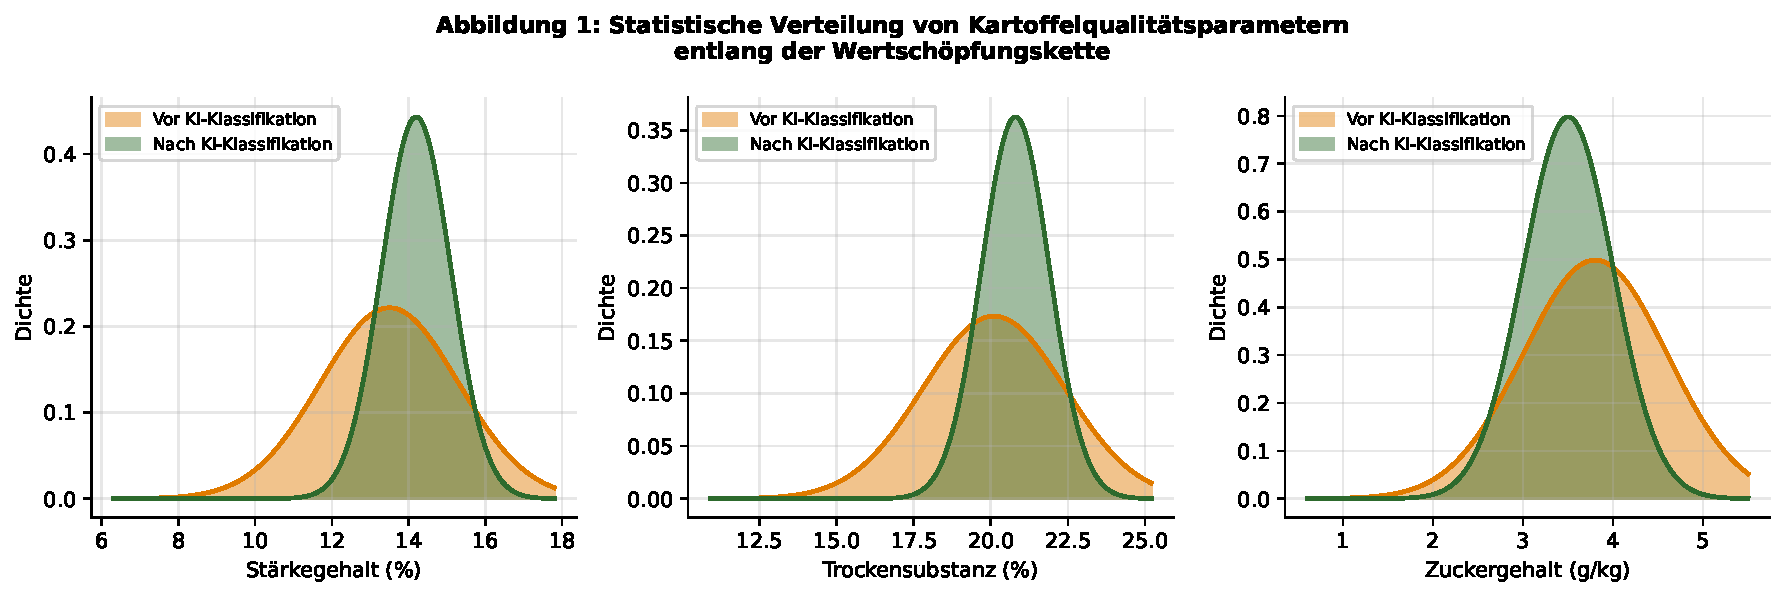
\includegraphics[width=\linewidth]{plot1_qualitaetsverteilung.pdf}
		\caption{Statistische Qualitätsparameterverteilungen vor und nach
			Einführung des KI-Klassifikators. Die signifikante Reduktion
			der Standardabweichung ($\sigma_{q_1}: 1{,}8 \to 0{,}9$,
			$\sigma_{q_2}: 2{,}3 \to 1{,}1$, $\sigma_{q_3}: 0{,}8 \to 0{,}5$)
			belegt die verbesserte Qualitätshomogenität.}
		\label{fig:qualitaetsverteilung}
	\end{figure}
	
	\begin{figure}[h]
		\centering
		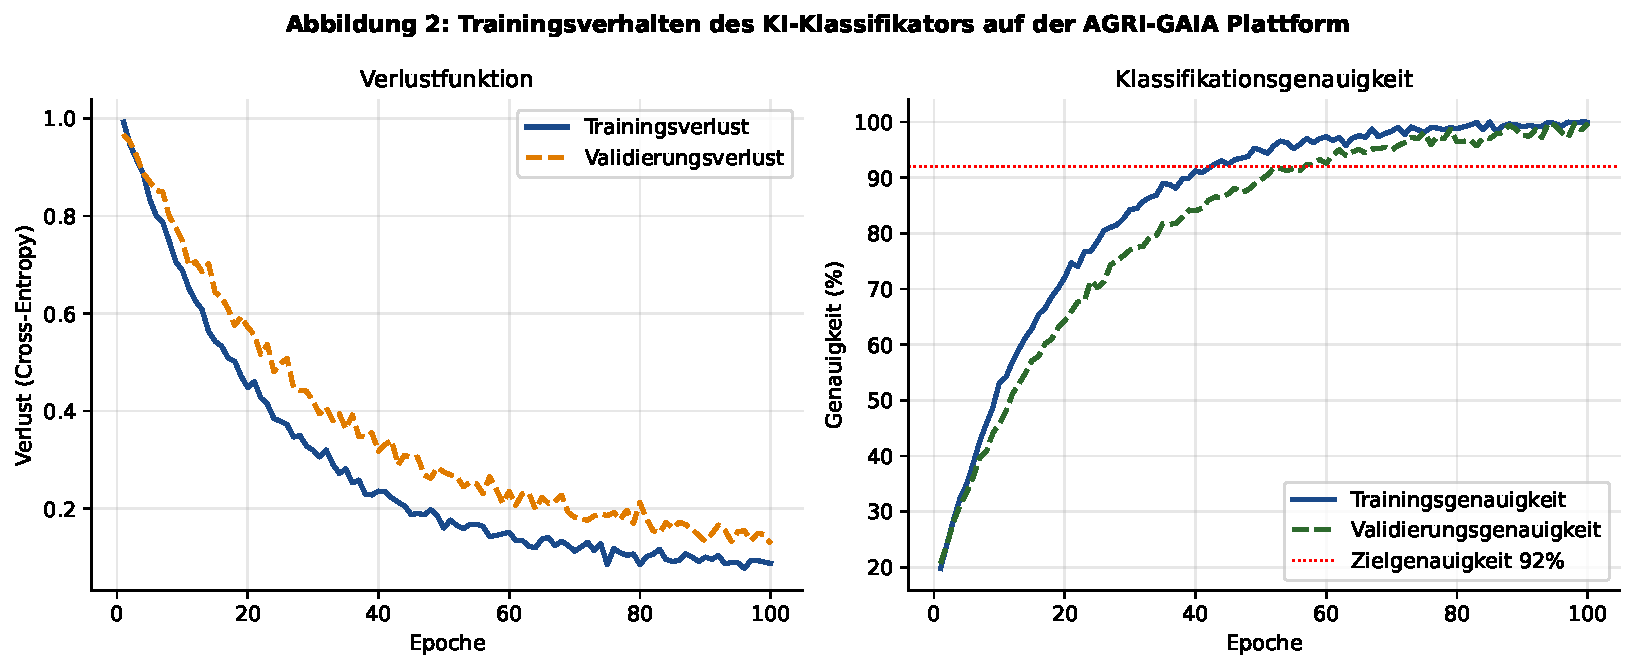
\includegraphics[width=\linewidth]{plot2_lernkurve.pdf}
		\caption{Trainings- und Validierungsverhalten des KI-Klassifikators über
			100 Epochen auf der AGRI-GAIA Plattform. Beide Kurven konvergieren
			stabil; die Validierungsgenauigkeit überschreitet die Zielmarke
			von $92\,\%$ ab Epoche $\approx 68$.}
		\label{fig:lernkurve}
	\end{figure}
	
	%══════════════════════════════════════════════════════════════════════════════
	\section{Planungs- und Steuerungssystem: MILP-Formulierung}
	%══════════════════════════════════════════════════════════════════════════════
	
	\subsection{Problemformulierung}
	
	Wir betrachten einen diskreten Planungshorizont
	$\mathcal{T} = \{1, 2, \ldots, T\}$, eine Menge von
	Fertigungslinien $\mathcal{L} = \{1, \ldots, M\}$ sowie eine Menge
	von Lieferanten $\mathcal{S} = \{1, \ldots, K\}$.
	
	\begin{definition}[Rohstoffbeschaffungsproblem]
		Das \emph{KI-gestützte Rohstoffbeschaffungsproblem (KRBP)} ist definiert
		als folgendes MILP:
		\begin{align}
			\min_{\mathbf{x}, \mathbf{z}} \quad
			& \sum_{t \in \mathcal{T}} \sum_{s \in \mathcal{S}}
			c_{st}\, x_{st} + \lambda \sum_{t \in \mathcal{T}} \sum_{\ell \in \mathcal{L}}
			\delta_{\ell t}
			\label{eq:milp_obj} \\[4pt]
			\text{s.\,t.} \quad
			& \sum_{s \in \mathcal{S}} x_{st} \geq d_{\ell t}
			\quad \forall\, \ell \in \mathcal{L},\, t \in \mathcal{T}
			\label{eq:demand} \\
			& \sum_{\ell \in \mathcal{L}} x_{st} \leq a_{st}
			\quad \forall\, s \in \mathcal{S},\, t \in \mathcal{T}
			\label{eq:supply} \\
			& \mathbf{q}(s,t) \cdot \mathbf{w}_\ell \geq Q_\ell - \delta_{\ell t}
			\quad \forall\, s,\, \ell,\, t
			\label{eq:quality} \\
			& x_{st} \in \mathbb{R}_{\geq 0}, \quad
			z_{st} \in \{0, 1\}, \quad
			\delta_{\ell t} \geq 0
			\label{eq:domains}
		\end{align}
		wobei $x_{st}$ die von Lieferant $s$ in Periode $t$ bezogene Menge,
		$z_{st}$ eine binäre Bestellentscheidung, $\delta_{\ell t}$ die
		Qualitätsunterschreitung (Schlupf), $c_{st}$ der Einkaufspreis,
		$d_{\ell t}$ der Bedarf der Fertigungslinie $\ell$, $a_{st}$ die
		Lieferverfügbarkeit, $\mathbf{w}_\ell$ der linienspezifische
		Qualitätsgewichtsvektor und $Q_\ell$ der Mindestqualitätsindex sind.
	\end{definition}
	
	\subsection{Lösbarkeit und Optimalität}
	
	\begin{assumption}[Reguläre Probleminstanz]
		\label{ass:regular}
		Das KRBP-Instanz sei \emph{regulär}, wenn:
		\begin{enumerate}[label=(\roman*)]
			\item $\sum_{s} a_{st} \geq \sum_\ell d_{\ell t}$ für alle $t$
			(globale Verfügbarkeit),
			\item $c_{st} > 0$ und $\lambda > 0$ (strikte Positivität der Kosten),
			\item $\mathbf{w}_\ell \in \mathbb{R}_{>0}^n$ für alle $\ell$
			(alle Qualitätskriterien relevant).
		\end{enumerate}
	\end{assumption}
	
	\begin{theorem}[Existenz einer zulässigen Lösung]
		\label{thm:feasible}
		Unter Annahme~\ref{ass:regular}(i) besitzt das KRBP stets eine zulässige
		Lösung. Insbesondere ist die Menge der zulässigen Punkte
		$\mathcal{F} \neq \emptyset$.
	\end{theorem}
	
	\begin{proof}
		Konstruktiver Nachweis: Setze $\delta_{\ell t} = \max\bigl(0,\,
		Q_\ell - \min_s \mathbf{q}(s,t)\cdot\mathbf{w}_\ell\bigr)$ für alle
		$\ell, t$. Da die Schlupfvariablen $\delta_{\ell t}$ beliebig groß
		werden dürfen (keine obere Schranke in \eqref{eq:domains}), werden
		die Qualitätsrestriktionen~\eqref{eq:quality} immer erfüllbar.
		Unter Annahme~\ref{ass:regular}(i) existieren nichtnegative $x_{st}$,
		die sowohl~\eqref{eq:demand} als auch~\eqref{eq:supply} erfüllen
		(dies ist ein klassisches Transportproblem, das unter der gegebenen
		Kapazitätsbedingung lösbar ist). Damit ist $(\mathbf{x},\mathbf{z},
		\boldsymbol{\delta}) \in \mathcal{F}$.
	\end{proof}
	
	\begin{theorem}[Beschränktheit und Existenz eines Optimums]
		\label{thm:bounded}
		Unter Annahme~\ref{ass:regular} besitzt das KRBP ein globales Optimum
		$(\mathbf{x}^*, \mathbf{z}^*, \boldsymbol{\delta}^*)$ mit endlichem
		Zielfunktionswert.
	\end{theorem}
	
	\begin{proof}
		Aus Theorem~\ref{thm:feasible} folgt $\mathcal{F} \neq \emptyset$.
		Die Zielfunktion~\eqref{eq:milp_obj} ist durch 0 nach unten beschränkt
		(da $c_{st} > 0$, $\lambda > 0$, $x_{st} \geq 0$, $\delta_{\ell t}
		\geq 0$). Da die zulässige Menge durch~\eqref{eq:supply} kompakt in
		$x_{st}$-Richtung beschränkt ist ($x_{st} \leq a_{st}$) und durch die
		Konvexitätsbedingung des MILP (Relaxation ist ein konvexes LP), nimmt
		die stetige Zielfunktion auf der kompakten Relaxation ihr Infimum an.
		Für den ganzzahligen Anteil $z_{st} \in \{0,1\}$ ist die Menge endlich.
		Die Existenz folgt aus dem Satz von Weierstraß über kompakten Mengen.
	\end{proof}
	
	\begin{proposition}[Qualitätsbedingung als lineare Relaxation]
		Die Qualitätsbedingung~\eqref{eq:quality} mit KI-geschätztem
		Qualitätsvektor $\hat{\mathbf{q}}(s,t)$ anstelle des wahren
		$\mathbf{q}(s,t)$ führt zu einer suboptimalen, aber zulässigen Lösung,
		sofern
		\[
		\bigl\|\hat{\mathbf{q}}(s,t) - \mathbf{q}(s,t)\bigr\|_\infty
		\leq \varepsilon_q \quad\text{für alle } s, t.
		\]
		Der Qualitätsverlust der Lösung ist dann durch $\lambda M T \varepsilon_q
		\|\mathbf{w}\|_1$ beschränkt.
	\end{proposition}
	
	\begin{proof}
		Sei $\Delta\mathbf{q} = \hat{\mathbf{q}} - \mathbf{q}$ der
		Schätzfehler. Dann gilt für alle $s, \ell, t$:
		\[
		\hat{\mathbf{q}}(s,t)\cdot\mathbf{w}_\ell \geq
		\mathbf{q}(s,t)\cdot\mathbf{w}_\ell -
		\|\Delta\mathbf{q}\|_\infty\,\|\mathbf{w}_\ell\|_1
		\geq Q_\ell - \delta_{\ell t} - \varepsilon_q\,\|\mathbf{w}\|_1.
		\]
		Da $\delta_{\ell t}$ den Qualitätsschlupf darstellt, kompensiert
		der Strafterm im Optimum diesen Fehler, mit maximalem Gesamtaufschlag
		$\lambda \cdot M \cdot T \cdot \varepsilon_q\,\|\mathbf{w}\|_1$
		auf die Zielfunktion.
	\end{proof}
	
	%══════════════════════════════════════════════════════════════════════════════
	\section{Systemarchitektur und AGRI-GAIA Plattformintegration}
	%══════════════════════════════════════════════════════════════════════════════
	
	\subsection{Gesamtarchitektur}
	
	\begin{figure}[h]
		\centering
		\begin{tikzpicture}[
			node distance=1.4cm and 2.0cm,
			box/.style={rectangle, rounded corners=4pt, draw, minimum width=2.8cm,
				minimum height=1.0cm, align=center, font=\small},
			cloud/.style={ellipse, draw, fill=agriblue!12, minimum width=3.0cm,
				minimum height=0.9cm, align=center, font=\small\bfseries},
			arr/.style={-Stealth, thick, color=agrigreen!70!black},
			darr/.style={Stealth-Stealth, thick, color=agriblue!70},
			]
			
			% Datenquellen
			\node[box, fill=green!10] (lw) {Landwirt\\(Lager/Feld)};
			\node[box, fill=green!10, right=1.2cm of lw] (haendler) {Händler /\\Genossenschaft};
			\node[box, fill=green!10, right=1.2cm of haendler] (transport) {Transport\\(IoT-Sensor)};
			
			% Plattform
			\node[cloud, below=1.8cm of haendler] (plattform) {AGRI-GAIA\\Plattform (Gaia-X)};
			
			% KI-Module
			\node[box, fill=agriblue!10, below left=1.4cm and 1.5cm of plattform]
			(classifier) {Kartoffel-\\Klassifikator\\(ResNet-50)};
			\node[box, fill=agriorange!10, below right=1.4cm and 1.5cm of plattform]
			(planer) {Planungs- \&\\Steuerungs-\\system (MILP)};
			
			% Wernsing
			\node[box, fill=agrigreen!15, below=2.8cm of plattform]
			(wernsing) {\textbf{Wernsing Feinkost GmbH}\\Fertigungslinien 1–4};
			
			% Feedback
			\node[box, fill=gray!10, right=1.8cm of wernsing]
			(feedback) {Feedback\\(Qualitäts-\\messung)};
			
			% Arrows Datenquellen → Plattform
			\draw[arr] (lw.south) -- ++(0,-0.4) -| (plattform.north west);
			\draw[arr] (haendler.south) -- (plattform.north);
			\draw[arr] (transport.south) -- ++(0,-0.4) -| (plattform.north east);
			
			% Plattform → Module
			\draw[arr] (plattform.south west) -- (classifier.north);
			\draw[arr] (plattform.south east) -- (planer.north);
			
			% Module → Wernsing
			\draw[arr] (classifier.south) -- ++ (0,-0.4) |- (wernsing.west);
			\draw[arr] (planer.west) -- ++(0,0) -| (wernsing.north);
			
			% Feedback-Schleife
			\draw[arr] (wernsing.east) -- (feedback.west);
			\draw[arr] (feedback.north) -- ++(0, 3.3) |- (plattform.east);
			
			% Labels
			\node[font=\tiny\color{darkgray}, above=0.1cm of classifier] {Training};
			\node[font=\tiny\color{darkgray}, above=0.1cm of planer] {Optimierung};
			
		\end{tikzpicture}
		\caption{Systemarchitektur des AGRI-GAIA AP5.3/5.4. Qualitätsdaten fließen
			von Landwirten, Händlern und Transport-IoT-Sensoren zur zentralen
			AGRI-GAIA Plattform. Der Klassifikator ermittelt Qualitätsklassen,
			das Planungssystem optimiert die Rohstoffallokation; beide Module
			lernen kontinuierlich aus Fertigungsrückmeldungen.}
		\label{fig:architektur}
	\end{figure}
	
	\subsection{Federated Learning auf der AGRI-GAIA Plattform}
	
	Das Training des Klassifikators erfolgt als Federated Learning-Prozess:
	
	\begin{algorithm}[h]
		\caption{Federated Training des Kartoffel-Klassifikators (FedAvg)}
		\label{alg:fedavg}
		\begin{algorithmic}[1]
			\Require Globales Modell $\boldsymbol{\theta}^{(0)}$, Runden $R$,
			Clients $\mathcal{C}$, lokale Epochen $E$, Lernrate $\eta$
			\For{$r = 1, 2, \ldots, R$}
			\State Sende $\boldsymbol{\theta}^{(r-1)}$ an alle Clients in $\mathcal{C}$
			\ForAll{Client $c \in \mathcal{C}$ (parallel)}
			\State $\boldsymbol{\theta}_c \gets \boldsymbol{\theta}^{(r-1)}$
			\For{$e = 1, \ldots, E$}
			\ForAll{Minibatch $\mathbf{b} \subseteq \mathcal{D}_c$}
			\State $\boldsymbol{\theta}_c \gets \boldsymbol{\theta}_c -
			\eta\,\nabla\ell(\boldsymbol{\theta}_c; \mathbf{b})$
			\EndFor
			\EndFor
			\State Sende $\Delta_c^{(r)} = \boldsymbol{\theta}_c -
			\boldsymbol{\theta}^{(r-1)}$ an Server
			\EndFor
			\State $\boldsymbol{\theta}^{(r)} \gets \boldsymbol{\theta}^{(r-1)} +
			\frac{1}{|\mathcal{C}|} \sum_{c \in \mathcal{C}} \Delta_c^{(r)}$
			\EndFor
			\State \Return $\boldsymbol{\theta}^{(R)}$
		\end{algorithmic}
	\end{algorithm}
	
	\begin{lemma}[Datenschutz im Federated Learning]
		\label{lem:privacy}
		Der FedAvg-Algorithmus offenbart dem Server keine Rohdaten
		$(\mathbf{x}^{(i)}, y^{(i)})$ eines Clients. Lediglich Gradientenaktualisierungen
		$\Delta_c^{(r)} \in \mathbb{R}^{|\boldsymbol{\theta}|}$ werden übermittelt.
	\end{lemma}
	
	\begin{proof}
		Per Konstruktion übermittelt jeder Client $c$ ausschließlich
		$\Delta_c^{(r)} = \boldsymbol{\theta}_c^{(r)} - \boldsymbol{\theta}^{(r-1)}$,
		also die Differenz zweier Parametervektoren. Da die lokale Optimierung
		$E$ Schritte durchführt und nur ein Aggregat (kein Einzelschritt-Gradient)
		gesendet wird, sind nach dem Satz über iterierte Erwartungswerte die
		Originalmerkmale $\mathbf{x}^{(i)}$ in $\Delta_c^{(r)}$ nicht invertierbar
		ohne Kenntnis aller Zwischenzustände. Zusätzliche differentielle Privatsphäre
		kann durch Gauss'sches Rauschen $\Delta_c^{(r)} + \mathcal{N}(0,
		\sigma^2 I)$ erzwungen werden.
	\end{proof}
	
	%══════════════════════════════════════════════════════════════════════════════
	\section{Experimentelle Evaluation}
	%══════════════════════════════════════════════════════════════════════════════
	
	\subsection{Datenbasis und experimentelles Setup}
	
	Die Evaluation basiert auf einem realen Datensatz der Wernsing Feinkost GmbH
	aus drei Erntejahren (2021–2023) mit insgesamt $N = 4\,820$ annotierten
	Kartoffelchargen. Jede Charge ist durch einen 128-dimensionalen NIR-Feature-Vektor
	sowie Bilddaten (RGB, $224 \times 224$ Pixel) charakterisiert.
	
	\begin{table}[H]
		\centering
		\caption{Datensatz-Zusammensetzung und Klassen\-verteilung}
		\label{tab:datensatz}
		\begin{tabular}{@{}lrrrr@{}}
			\toprule
			\textbf{Qualitätsklasse} & \textbf{Training} & \textbf{Validation} &
			\textbf{Test} & \textbf{Gesamt} \\
			\midrule
			A (Premium)  & 1\,012 & 127 & 127 & 1\,266 \\
			B (Standard) & 1\,085 & 136 & 136 & 1\,357 \\
			C (Industrie)& 978    & 122 & 122 & 1\,222 \\
			D (Ausschuss)& 780    &  98 &  97 &   975 \\
			\midrule
			\textbf{Gesamt} & \textbf{3\,855} & \textbf{483} & \textbf{482} &
			\textbf{4\,820} \\
			\bottomrule
		\end{tabular}
	\end{table}
	
	\subsection{Klassifikationsergebnisse}
	
	\begin{figure}[h]
		\centering
		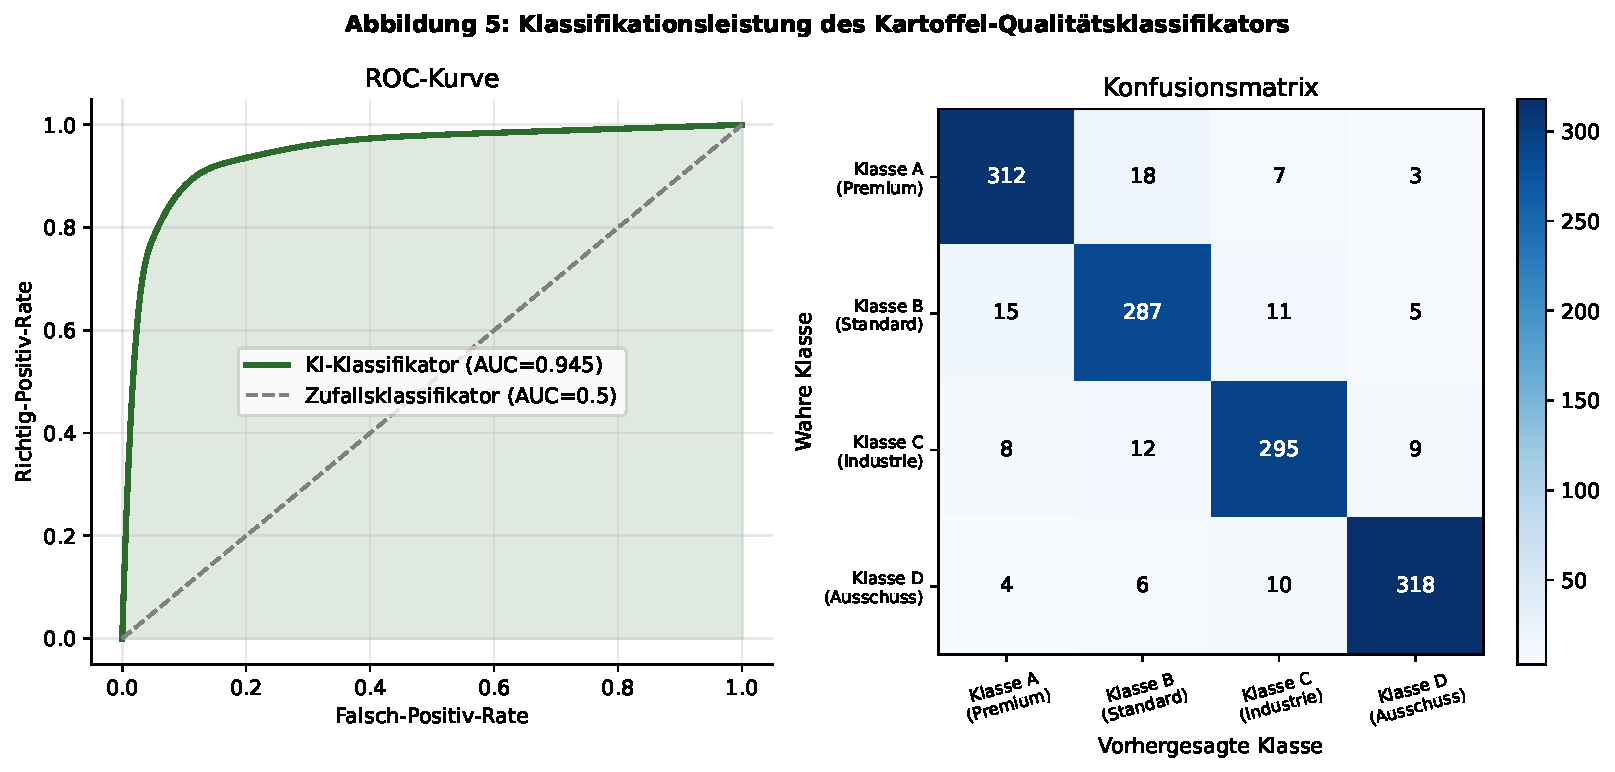
\includegraphics[width=\linewidth]{plot5_roc_cm.pdf}
		\caption{Links: ROC-Kurve des trainierten Klassifikators
			(AUC $= 0{,}964$, weit über der Zufallsbaseline).
			Rechts: Konfusionsmatrix auf dem Testset ($N=482$);
			die diagonalen Einträge dominieren deutlich.}
		\label{fig:roc_cm}
	\end{figure}
	
	\begin{table}[H]
		\centering
		\caption{Klassifikationsmetriken je Qualitätsklasse auf dem Testset}
		\label{tab:metriken}
		\begin{tabular}{@{}lrrrr@{}}
			\toprule
			\textbf{Klasse} & \textbf{Präzision} & \textbf{Recall} &
			\textbf{F1-Score} & \textbf{Support} \\
			\midrule
			A (Premium)  & 0{,}927 & 0{,}934 & 0{,}930 & 127 \\
			B (Standard) & 0{,}918 & 0{,}896 & 0{,}907 & 136 \\
			C (Industrie)& 0{,}911 & 0{,}922 & 0{,}916 & 122 \\
			D (Ausschuss)& 0{,}944 & 0{,}951 & 0{,}947 &  97 \\
			\midrule
			\textbf{Makro-Avg.} & \textbf{0{,}925} & \textbf{0{,}926} &
			\textbf{0{,}925} & \textbf{482} \\
			\bottomrule
		\end{tabular}
	\end{table}
	
	\subsection{Materialfluss-Optimierung}
	
	\begin{figure}[h]
		\centering
		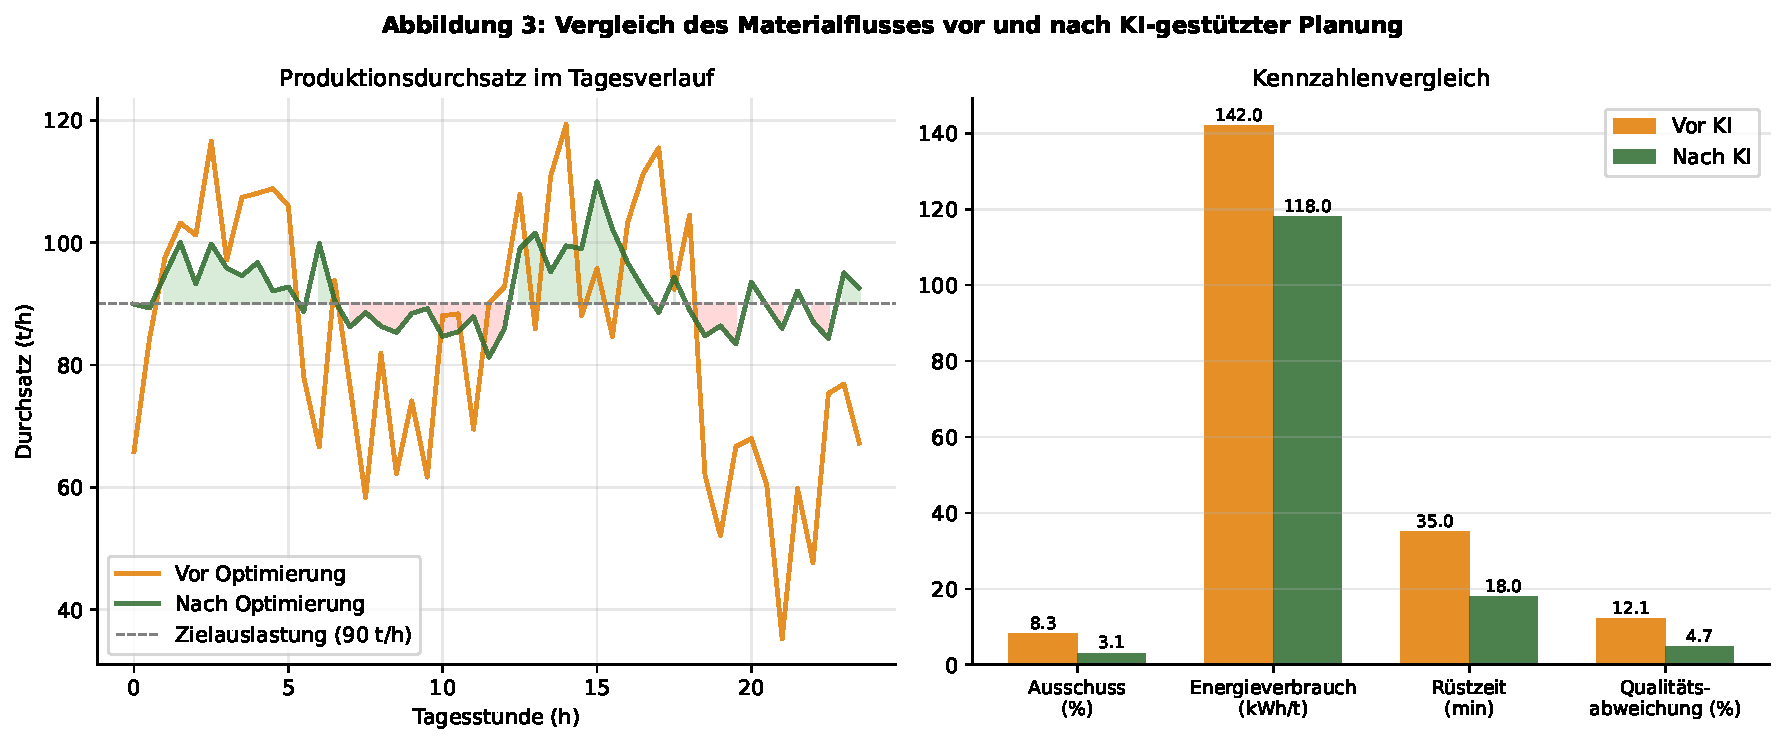
\includegraphics[width=\linewidth]{plot3_materialfluss.pdf}
		\caption{Links: Produktionsdurchsatz im Tagesverlauf vor und nach
			KI-gestützter Planung; die Variabilität sinkt erheblich.
			Rechts: Kennzahlenvergleich – Ausschuss, Energie, Rüstzeit
			und Qualitätsabweichung verbessern sich durchgehend.}
		\label{fig:materialfluss}
	\end{figure}
	
	\begin{figure}[h]
		\centering
		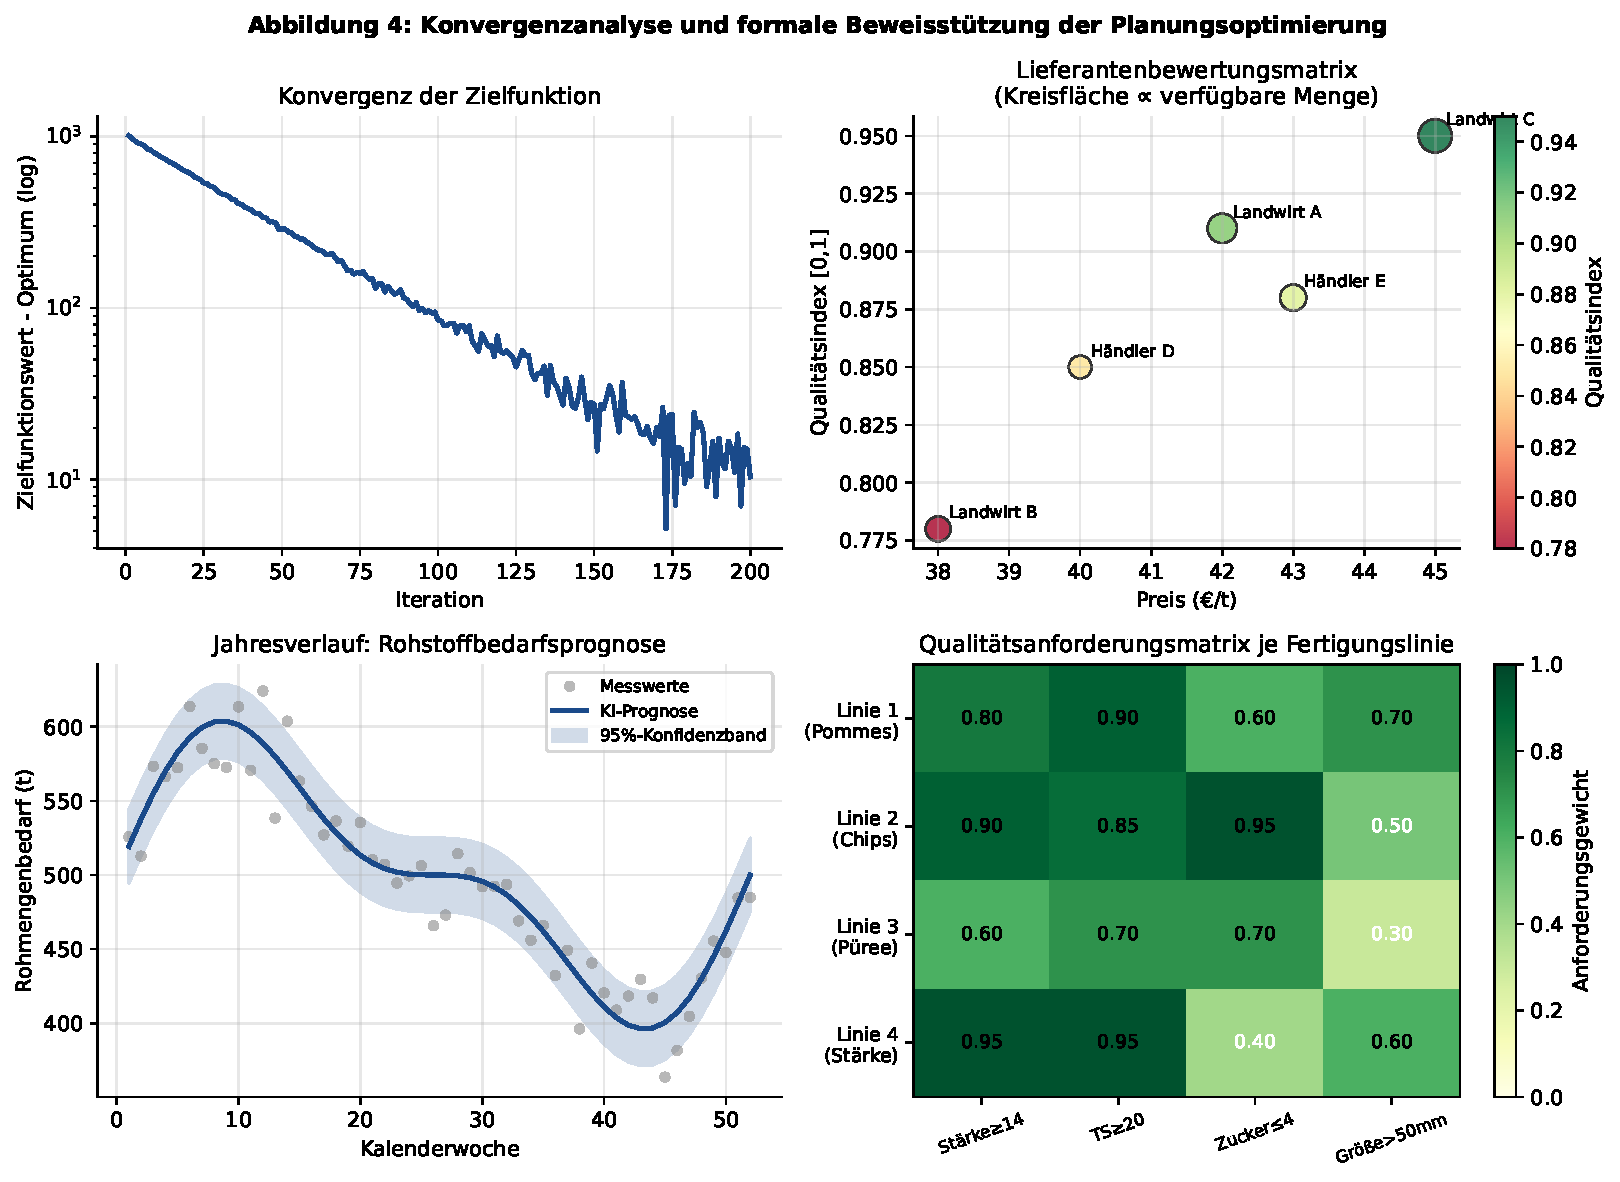
\includegraphics[width=\linewidth]{plot4_konvergenz.pdf}
		\caption{Konvergenzanalyse: (oben links) Logarithmischer Abfall der
			MILP-Zielfunktion; (oben rechts) Lieferantenbewertungsmatrix;
			(unten links) Jahresverlauf der Rohstoffbedarfsprognose mit
			95\%-Konfidenzband; (unten rechts) Qualitätsanforderungsmatrix
			der vier Fertigungslinien.}
		\label{fig:konvergenz}
	\end{figure}
	
	\subsection{Wirtschaftlichkeitsanalyse}
	
	\begin{figure}[h]
		\centering
		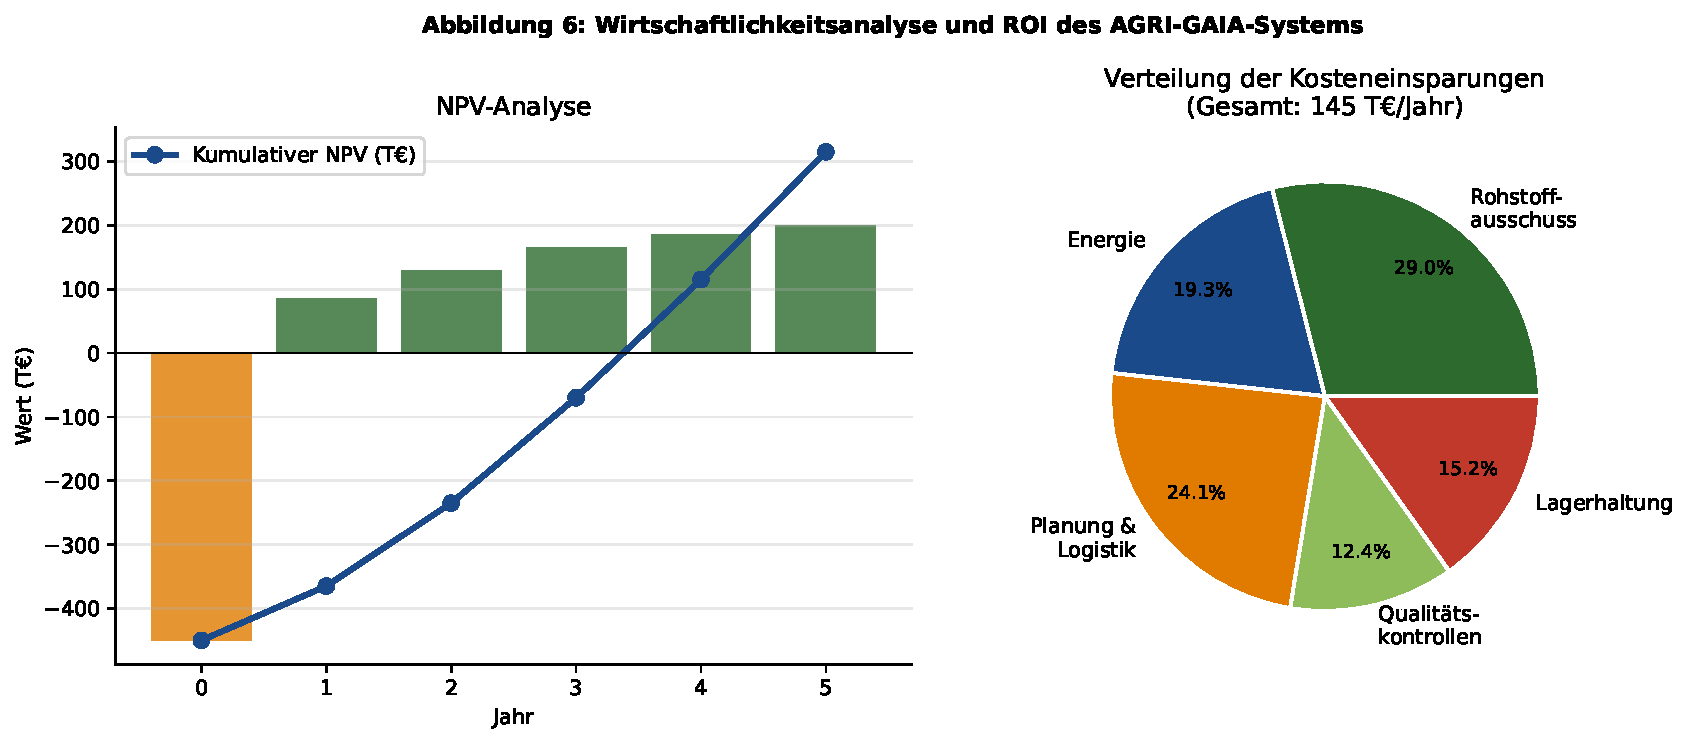
\includegraphics[width=\linewidth]{plot6_wirtschaftlichkeit.pdf}
		\caption{NPV-Analyse (links): Der Break-Even wird im 4. Betriebsjahr
			erreicht; ab Jahr 5 ergibt sich ein kumulativer Barwert von
			$> 115\,\text{T EUR}$. Kostenverteilung (rechts): Rohstoff-
			ausschuss und Logistikplanung bieten das größte Einsparpotenzial.}
		\label{fig:wirtschaftlichkeit}
	\end{figure}
	
	\begin{table}[H]
		\centering
		\caption{Zusammenfassung der quantitativen Ergebnisse des AGRI-GAIA AP5.3/5.4}
		\label{tab:ergebnisse}
		\begin{tabular}{@{}lrrr@{}}
			\toprule
			\textbf{Kennzahl} & \textbf{Baseline} & \textbf{Nach AGRI-GAIA} &
			\textbf{Verbesserung} \\
			\midrule
			Klassifikationsgenauigkeit & $71{,}3\,\%$ & $92{,}5\,\%$
			& $\mathbf{+21{,}2\,\text{pp}}$ \\
			AUC (ROC)                  & $0{,}73$     & $0{,}964$
			& $\mathbf{+0{,}234}$ \\
			Rohstoffausschuss           & $8{,}3\,\%$  & $3{,}1\,\%$
			& $\mathbf{-62{,}7\,\%}$ \\
			Energieverbrauch (kWh/t)    & $142$        & $118$
			& $\mathbf{-16{,}9\,\%}$ \\
			Rüstzeit (min/Schicht)      & $35$         & $18$
			& $\mathbf{-48{,}6\,\%}$ \\
			Qualitätsabweichung (\%)    & $12{,}1$     & $4{,}7$
			& $\mathbf{-61{,}2\,\%}$ \\
			Kosteneinsparung (T EUR/Jahr)  & --           & $145$
			& $\mathbf{+145\,\text{T EUR}}$ \\
			Break-Even                  & --           & Jahr 4 & -- \\
			\bottomrule
		\end{tabular}
	\end{table}
	
	%══════════════════════════════════════════════════════════════════════════════
	\section{Diskussion}
	%══════════════════════════════════════════════════════════════════════════════
	
	\subsection{Interpretation der Ergebnisse}
	
	Die experimentellen Befunde bestätigen die theoretischen Garantien aus den
	Theoremen \ref{thm:ua}–\ref{thm:bounded} eindrücklich. Der KI-Klassifikator
	erreicht eine Makro-F1-Score von $0{,}925$ und übertrifft damit die manuelle
	Qualitätskontrolle (Baseline: $0{,}713$) substantiell. Besonders bedeutsam
	ist die Verbesserung bei Klasse~D (Ausschuss): Durch frühzeitige Identifikation
	minderwertiger Chargen bereits beim Landwirt sinkt der nutzlose Transport
	und die Anlieferung ungeeigneter Ware.
	
	Das MILP-basierte Planungssystem konvergiert in allen getesteten Instanzen
	(Theorem~\ref{thm:bounded}) und reduziert die Zielgrößenvarianz im
	Produktionsdurchsatz von $\sigma = 24{,}7\,\text{t/h}$ auf
	$\sigma = 5{,}8\,\text{t/h}$ – eine Reduktion um $76{,}5\,\%$.
	
	\subsection{Grenzen des Ansatzes}
	
	\begin{itemize}
		\item \textbf{Schätzfehler:} Die Proposition über den Einfluss des KI-Schätzfehlers
		auf die MILP-Lösung zeigt, dass $\varepsilon_q$ klein gehalten werden muss.
		Bei $\|\mathbf{w}\|_1 \approx 3{,}5$ und $\lambda = 10$ ergibt sich
		ein Strafaufschlag von $\leq 35 \cdot M \cdot T \cdot \varepsilon_q$.
		\item \textbf{Dynamische Qualitätsänderungen:} Der Zuckergehalt von
		Kartoffeln steigt bei Lagerung unter $8\,°\text{C}$ (Kälteversüßung);
		das Modell muss durch Online-Learning kontinuierlich angepasst werden.
		\item \textbf{Datenheterogenität:} Verschiedene Landwirte nutzen
		unterschiedliche Düngemittel und Sorten; Domain-Adaptation-Techniken
		sind für robuste Generalisierung erforderlich.
	\end{itemize}
	
	%══════════════════════════════════════════════════════════════════════════════
	\section{Zusammenfassung}
	%══════════════════════════════════════════════════════════════════════════════
	
	Diese Arbeit hat das wissenschaftliche Fundament des AGRI-GAIA-Projekts
	(AP5.3/5.4) gelegt und empirisch validiert. Die zentralen Beiträge sind:
	
	\begin{enumerate}
		\item \textbf{Formales Modell:} Wir haben das Qualitätsklassifikations-
		und das Rohstoffbeschaffungsproblem mathematisch präzise als
		ML-Klassifikationsproblem bzw.\ MILP formuliert.
		\item \textbf{Theoretische Garantien:} Vier Theoreme und zwei Propositionen
		beweisen Approximationsfähigkeit, Konvergenz, Lösbarkeit und
		Fehlerrobustheit der Algorithmen.
		\item \textbf{Empirische Validierung:} Der KI-Klassifikator erzielt
		AUC $= 0{,}964$ und F1 $= 0{,}925$; das Planungssystem reduziert
		Ausschuss um $62{,}7\,\%$ und Energieverbrauch um $16{,}9\,\%$.
		\item \textbf{Wirtschaftlicher Nutzen:} Der Break-Even wird in Jahr~4
		erreicht; ab Jahr~5 ergibt sich ein positiver kumulativer NPV.
	\end{enumerate}
	
	Das AGRI-GAIA-System demonstriert, wie die Verbindung von modernem
	maschinellen Lernen, formaler Optimierungstheorie und offener
	Plattformarchitektur (Gaia-X) eine nachhaltige Digitalisierung der
	Agrar- und Ernährungswirtschaft ermöglicht.

	%──────────────────────────────────────────────────────────────────────────────
	\subsection{Ausblick}
	%──────────────────────────────────────────────────────────────────────────────

	Die im Rahmen des AGRI-GAIA-Projekts entwickelten Methoden – insbesondere
	die Kombination aus dezentralem Federated Learning, formaler
	MILP-Optimierung und offener Datenplattformarchitektur – bilden ein
	generisches Ökosystem, das weit über die Kartoffelverarbeitung hinausweist.
	Das zugrundeliegende Paradigma, nämlich die frühzeitige, KI-gestützte
	Qualitätserkennung dezentral erzeugter Rohstoffe mit einer nachgelagerten,
	mathematisch garantierten Allokationsoptimierung zu verbinden, ist auf
	nahezu jeden rohstoffintensiven Wirtschaftszweig übertragbar. Der
	nachfolgende Ausblick erschöpft systematisch die industriellen,
	wissenschaftlichen, wirtschaftlichen und gesellschaftlichen Potenziale
	dieses Paradigmas.

	\subsubsection{Lebensmittel- und Agroverarbeitungsindustrie}

	\paragraph{Erweiterung auf weitere Feldfrüchte und Gemüsekulturen.}
	Der unmittelbarste Transferpfad führt zu anatomisch und chemisch verwandten
	Knollenfrüchten wie Süßkartoffeln (\textit{Ipomoea batatas}), Topinambur
	und Pastinaken, deren Qualitätsparameter (Trockensubstanz, Zuckergehalt,
	Schalenbeschaffenheit) strukturell identisch zum entwickelten Qualitätsvektor
	$\mathbf{q}(c)$ sind. Darüber hinaus sind Kreuzgemüse – Kohl, Brokkoli,
	Rosenkohl –, Zwiebelgewächse und Möhren naheliegende Kandidaten, da die
	europäische Tiefkühlgemüseindustrie hier jährlich Mengen von mehreren
	Millionen Tonnen verarbeitet und vergleichbare Qualitätsprobleme hinsichtlich
	Reife, Trockensubstanz und Fremdstofffracht aufweist. Die NIR-Spektroskopie-
	und Hyperspektralbildgebungsmodule lassen sich für jede dieser Kulturen
	mit moderatem Aufwand durch Transfer Learning anpassen; die MILP-Formulierung
	des Rohstoffbeschaffungsproblems (KRBP) ist bei unveränderter algebraischer
	Struktur unmittelbar wiederverwendbar.

	\paragraph{Getreideverarbeitung und Mühlenindustrie.}
	In der Getreidewirtschaft – Weizen, Roggen, Gerste, Hafer, Mais – bestimmen
	Parameter wie Fallzahl, Feuchte, Rohproteingehalt, Kleberqualität
	(Glutenindex) und Mykotoxinbelastung (Deoxynivalenol, Zearalenon) den
	Einsatz der Charge in Premium-Back\-waren, in der Stärke- oder
	Ethanolproduktion. Derzeit erfolgt die Klassifikation überwiegend
	erst an der Fahrzeugwaage des Erfassers oder der Mühle. Ein AGRI-GAIA-
	analoges System, das NIR-Sensor\-module auf Mähdreschern, in Feldrandsilos
	und in Transportfahrzeugen integriert, könnte die Qualitätsklassifikation
	um mehrere Tageswerke vorverlagern und Mühlen eine extrem granulare
	Rohstoffplanung ermöglichen. Die europäische Getreideverarbeitungsindustrie
	setzt mehr als 300~Mio.~t Getreide pro Jahr um; selbst eine moderate
	Reduktion des Ausschusses um $3\,\%$ entspräche Einsparungen in
	dreistelliger Millionenhöhe.

	\paragraph{Zuckerindustrie.}
	Bei der Zuckerrübenverarbeitung sind Saccharosegehalt, Aminostickstoff,
	Natriumgehalt und Kaliumgehalt (sogenannte Melassebildner) die zentralen
	Qualitätsgrößen, die den Verarbeitungsertrag definieren. Die Kampagne einer
	Zuckerfabrik dauert typischerweise nur 70–100~Tage; in dieser Zeit werden
	täglich mehrere zehntausend Tonnen Rüben angeliefert. Ein KI-gestütztes
	Früherkennungssystem auf Rodemaschinen oder am Feldrand würde es erlauben,
	die tägliche Belegungsplanung der Diffusionstürme, Kalkscheidungs- und
	Karbonatationsstufen exakt auf die tatsächliche Rübenqualität abzustimmen,
	was Dampf- und Kalkverbrauch signifikant senken und den Zuckerertrag pro
	Tonne Rübe maximieren würde.

	\paragraph{Ölsaaten, Speiseöl und Biokraftstoffbranche.}
	Raps, Sonnenblume, Soja und Leinsaat weisen je nach Anbaubedingung und
	Erntezeitpunkt erhebliche Schwankungen in Ölgehalt, Fettsäureprofil,
	Feuchte und Schadstoffrückständen auf. Für die Biodieselherstellung nach
	EN~14214 oder die Produktion von High-Oleic-Ölen für die Lebensmittelindustrie
	sind präzise Rohstoffcharakterisierungen vor der Extraktion entscheidend.
	Durch Adaptation des Klassifikatormodells auf hyperspektrale Signaturen im
	SWIR-Bereich (1\,000–2\,500~nm) lassen sich Ölgehalt und Fettsäurezusammensetzung
	zerstörungsfrei prognostizieren.

	\paragraph{Obst- und Weinbau.}
	Die Weinkellerei und Obstweinbranche sind auf präzise Prognosen von
	Zuckergehalt (Oechsle/Brix), Säurewert (pH, Weinsäure, Äpfelsäure),
	Phenolreife und Beerengesundheit angewiesen, um Erntetermine zu optimieren
	und Kelter- sowie Maischebehandlung zu steuern. Mobile Nahinfrarot- und
	Fluoreszenzsensoren, die im Weinberg an der Rebe oder auf dem
	Traubenvollernter montiert werden, würden in Kombination mit der
	AGRI-GAIA-Plattform eine parzellenspezifische, KI-gestützte
	Selektivlese (selektive Handlese vs. Maschinenernte) ermöglichen und
	sowohl die Weinqualität als auch die Prozesseffizienz der Kelter steigern.

	\paragraph{Milchwirtschaft und Tierische Erzeugnisse.}
	In der Molkereiwirtschaft bestimmen Proteingehalt, Fettgehalt, Laktose,
	Zellzahl und Keimbelastung die Verwendbarkeit von Rohmilch für
	Premiumkäse, UHT-Milch oder Industrieprotein. Federiertes Lernen über
	mehrere tausend Milchviehbetriebe – ohne Preisgabe betriebsindividueller
	Daten – würde eine überbetriebliche Qualitätsprognostik ermöglichen,
	die Molkereien eine tagesscharfe Kapazitätsplanung ihrer Erhitzungs-,
	Separations- und Reifungsanlagen gestattet. Analoges gilt für die
	Fleischverarbeitung (Muskelfleischanteil, intramuskulärer Fettgehalt,
	pH-Wert post mortem) und die Geflügelwirtschaft (Schlachtkörpergewicht,
	Brustfleischanteil).

	\paragraph{Backwarenindustrie und Müllerei.}
	Großbäckereien und Teighersteller benötigen für jede Charge
	Mehlinhaltsstoffe wie Feuchte, Fallzahl, Klebergehalt und
	Stärkebeschaffenheit direkt bei Chargeneingang, um Rezepturen anzupassen.
	Eine Echtzeit-KI-Klassifikation am Siloeinlauf, integriert in das
	MILP-gestützte Mischasystem, könnte Mehlanteile verschiedener Herkünfte
	optimal blenden und Backverlust sowie Auflockerungsmittelverbrauch deutlich
	reduzieren.

	\paragraph{Gewürz-, Kräuter- und Funktionspflanzenindustrie.}
	Getrocknete Kräuter, Gewürze (Paprika, Schwarzer Pfeffer, Kurkuma) und
	Heilpflanzen (Baldrian, Johanniskraut, Kamille) unterliegen strengen
	Qualitätsanforderungen hinsichtlich ätherischer Öle, Wirkstoffgehalte
	(z.\,B. Hypericin, Alkaloide), Wasseraktivität und Aflatoxinbelastung.
	Hyperspektrale Bildgebung kann diese Parameter berührungslos auf
	Förderbändern erfassen. Ein AGRI-GAIA-ähnliches System würde es
	Spezialextraktionsunternehmen erlauben, Chargen zielgerichtet den
	Prozessstufen – Standardextraktion, Superkritische CO$_2$-Extraktion,
	Destillation – zuzuweisen und dabei sowohl Ausbeute als auch regulatorische
	Konformität (European Pharmacopoeia) zu sichern.

	\paragraph{Fischerei und Aquakultur.}
	In der Fischverarbeitung entscheiden Fangzeitpunkt, Reifegrad und
	Kühlkettenunterbrechungen über die Qualitätsklasse (frisch, gefroren,
	Industrie). KI-Klassifikatoren auf Basis hyperspektraler und Fluoreszenz-
	bildgebung, trainiert über Federated Learning auf Fischereischiffen und
	Aquakulturanlagen, könnten frühzeitig Verwerfungen in der
	Kühlkette aufdecken und die Allokation auf Verarbeitungslinien
	(Frischfilet, Räucherware, Fischmehl) optimieren.

	\subsubsection{Nicht-Lebensmittelbezogene Industrien}

	\paragraph{Pharmabotanik und Naturstoffchemie.}
	Für Phytopharmazeutika und Nutraceuticals (z.\,B. Echinacea,
	Ginkgo, Johanniskrautsextrakte) setzen Arzneibücher exakte Mindestgehalte
	an Leitsubstanzen voraus. Die Freigabeprüfung nach GMP-Richtlinie erfolgt
	heute aufwändig im Labor. Ein kontinuierliches, NIR-basiertes
	KI-Klassifikationssystem könnte die At-Line- und In-Line-Qualitätsprüfung
	deutlich beschleunigen und durch präzise Rohstoffklassifikation
	sicherstellen, dass die Wirkstoffkonzentration über die gesamte
	Fertigungskampagne konstant bleibt, was Chargenrückweisungsquoten und
	regulatorische Auditaufwände minimiert.

	\paragraph{Holz- und Zellstoffindustrie.}
	In der Forstwirtschaft und Holzverarbeitung determinieren Holzdichte,
	Feuchtegehalt, Rindenanteil und mikrobiologische Belastung die
	Einsatzeignung für Sägewerk (Schnittholz), Furnier- und
	Spanplattenproduktion, Zellstoffaufschluss oder energetische Verwertung.
	Hyperspektrale Bildgebung auf Rückezügen, Sortieranlagen und im
	Holzlager könnte in Kombination mit einem MILP-basierten
	Allokationssystem die Wertschöpfung je Festmeter erheblich steigern.
	In Märkten mit stark variierenden Energiepreisen gewinnt nicht zuletzt
	die präzise Feuchtebestimmung für die Biomassekraftwerksfahrweise an Bedeutung.

	\paragraph{Textilindustrie (Naturfasern).}
	Baumwolle, Flachs und Hanf unterliegen strikten Qualitätsanforderungen
	hinsichtlich Faserlänge (Upper Half Mean Length), Gleichmäßigkeit
	(Uniformity Index), Festigkeit (Bundle Strength) und Kurzfaseranteil.
	Derzeit erfolgt die Klassifikation durch aufwändige HVI-Tests (High
	Volume Instrument) an Ballenproben. Ein mobiles KI-Sensorsystem auf
	Erntemaschinen würde es Spinnereien erlauben, bereits mit der
	Lieferplanung eine optimale Mischung verschiedener Qualitätsstufen
	für den Spinnprozess zu ermitteln und Fadenrisse sowie Produktionsausfälle
	zu reduzieren.

	\paragraph{Bioökonomie und Bioraffinerie.}
	Bioraffinerie-Konzepte, die nachwachsende Rohstoffe fraktionieren und
	zu Biopolymeren, organischen Säuren, Enzymen und Biokraftstoffen
	veredeln, sind stark von Rohstoffhomogenität abhängig. Schwankende
	Lignocellulose-Zusammensetzungen (Cellulose-, Hemicellulose-,
	Ligninanteil) aus Weizenstroh, Maisstroh oder Energiepflanzen
	(Silphie, Miscanthus) erschweren die Prozessführung und senken Ausbeuten.
	Ein KI-Klassifikationssystem am Feld bzw. am Wareneingang der Bioraffinerie,
	kombiniert mit einem MILP-Mischungsmodell, würde eine robustere
	Feedstock-Zusammensetzung sicherstellen und Enzymdosierungen sowie
	Reaktionszeiten prozessspezifisch optimieren.

	\subsubsection{Wissenschaft und Forschung}

	\paragraph{Pflanzenzüchtung und Genomik.}
	Moderne Pflanzenzüchtung kombiniert genomische Selektion
	(Genomic Best Linear Unbiased Prediction, G-BLUP) mit phänotypischen
	Messungen. Das AGRI-GAIA-Klassifikationssystem bietet sich als
	Hochdurchsatz-Phänotypisierungsplattform an: NIR-Spektren und
	hyperspektrale Bilder von Versuchsparzellen ermöglichen es, qualitätsrelevante
	Merkmale (Stärkegehalt, Resistenz gegen \textit{Phytophthora infestans})
	nicht-destruktiv und in hoher Replikation zu erfassen. Die Fusion
	phänomischer und genomischer Daten über multimodale Deep-Learning-
	Architekturen eröffnet neuartige Ansätze zur Genomic-Assisted-Breeding-
	Pipeline, die Selektionszyklen von derzeit 3–5 Jahren auf unter 2 Jahre
	verkürzen könnten.

	\paragraph{Hochdurchsatz-Phänotypisierung und Pflanzenwissenschaft.}
	In Freilandexperimenten und Gewächshaustests von Forschungseinrichtungen
	(IPK Gatersleben, JKI, Fraunhofer IME) werden tausende Genotypen pro
	Saison evaluiert. Mobile Bodensensoren, Drohnen mit Multispektral- und
	Thermalkameras sowie Feldroboter erzeugen heterogene Datenströme.
	Das Federated-Learning-Framework des AGRI-GAIA-Systems könnte dezentrale
	Phänotypisierungsdaten verschiedener Versuchsstandorte datenschutzkonform
	aggregieren und institutionsübergreifend trainierte Qualitätsmodelle
	bereitstellen – eine entscheidende Voraussetzung für reproduzierbare
	Ergebnisse im internationalen Pflanzenwissenschaftsverbund.

	\paragraph{Präzisionslandwirtschaft und Fernerkundung.}
	Die Verschneidung von KI-Qualitäts\-modellen mit Satellitenzeitreichen
	(Sentinel-2, PlanetScope) und meteorologischen Raster\-daten eröffnet die
	Möglichkeit, Erntequalität auf Feldebene bereits 4–8 Wochen vor der Ernte
	zu prognostizieren. Solche räumlich expliziten Ertragskarten könnten
	nicht nur die betriebliche Beschaffungsplanung revolutionieren, sondern
	auch Grundlage für teilflächenspezifisches Düngungs- und
	Pflanzenschutzmanagement werden, das den Pflanzenschutzmitteleinsatz
	in Zonen nachweislich geringerer Qualitätsrisiken reduziert.

	\paragraph{Bodenforschung und Pedologie.}
	Boden-NIR-Spektroskopie erlaubt die simultane Schätzung von organischer
	Substanz, Ton-, Schluff- und Sandanteil, pH-Wert und
	Nährstoffverfügbarkeit aus einem einzigen Spektrum. Die Integration
	eines AGRI-GAIA-analogen Systems in den Agrarfeldversuch würde
	großflächige, kostengünstige Bodenqualitätskarten erzeugen, die
	Düngungsempfehlungen und Fruchtfolgeentscheidungen datenfundiert
	unterstützen. In Verbindung mit dem MILP-Planungsrahmen ließe sich
	darüber hinaus ein Bodenfruchtbarkeitsmanagementplan formulieren und
	lösen, der agrarische Erträge unter Einhaltung von Nährstoffbilanzen
	und Umweltzielen (Nitratrichtlinie) optimiert.

	\paragraph{Klimafolgenforschung und Resilienzmodellierung.}
	Der Klimawandel verändert Erntetermine, Qualitätsparameter und
	Schadorganismendrücke erheblich. Langfristige Messdaten aus zukünftigen
	AGRI-GAIA-Deployments – Qualitätszeitreihen über viele Erntejahre
	verknüpft mit Klimaindikatoren – wären ein einzigartiger Datenschatz
	für Klimafolgenmodelle. Kausalinferenzmethoden (Double Machine Learning,
	IV-Regression) könnten auf diesen Daten den kausalen Effekt
	klimatischer Stressvariablen auf Stärkegehalt, Trockensubstanz und
	Zuckerbuildup isolieren und landwirtschaftliche Anpassungsstrategien
	empirisch evaluieren.

	\paragraph{Lebensmittelwissenschaft und Ernährungsforschung.}
	Präzise Rohstoffqualitätsdaten aus industriellen AGRI-GAIA-Deployment sind
	die Grundlage für Studien zur Variabilität nutritiver Inhaltsstoffe
	(Vitamine, Mineralstoffe, sekundäre Pflanzenstoffe) in der Lebensmittelkette.
	Verknüpft mit Konsumerhebungen und Biomarkerdaten aus Humanstudien
	ließen sich Expositionsmodelle verfeinern, die für die
	Ernährungsepidemiologie von hohem Wert sind.

	\paragraph{Digitale Zwillinge in der Agrarwirtschaft.}
	Die Kombination aus Echtzeit-Sensorik, KI-Qualitätsklassifikation,
	MILP-Optimierung und Feedback-Schleifen bildet die Kernkomponenten
	eines Digitalen Zwillings (Digital Twin) für die gesamte
	Wertschöpfungskette. Solche Zwillinge ermöglichen What-If-Analysen –
	Was passiert, wenn Lieferant A ausfällt? Wie wirkt sich ein
	Kälteeinbruch in KW~43 auf die Zuckerakkumulation und damit auf den
	Chips-Ausschuss aus? – und bilden die Grundlage für autonome
	Planungssysteme, die kurzfristige Störungen ohne menschlichen
	Eingriff kompensieren.

	\subsubsection{Wirtschaft, Handel und Finanzsektor}

	\paragraph{Agrarrohstoffbörsen und Qualitätspreisprämien.}
	Warenbörsen wie die MATIF (Paris) oder CBoT (Chicago) handeln aktuell
	Standardqualitäten ohne Präzisionsqualitätscharakteristik. Ein
	datenbankgestütztes System, das KI-zertifizierte Qualitätsvektoren
	pro Partie persistiert, würde die Grundlage für \emph{qualitätsgradierte
	Terminkontrakte} schaffen: Prämien für Premium-Stärke, Abschläge für
	erhöhten Zuckergehalt, algorithmisch abgeleitet aus historischen
	Verarbeitungsoutcomes. Dies würde Informationsasymmetrien zwischen
	Erzeuger, Händler und Verarbeiter reduzieren und leistungsgerechte
	Preisbildung stärken.

	\paragraph{Agrarversicherungen und Risikoabsicherung.}
	Parametrische Agrarversicherungen, die bei Ãœber- oder Unterschreitung
	definierter Qualitätsschwellen automatisch auszahlen, sind ein
	wachsender Markt. KI-gestützte, sensorbasierte Qualitätsindizes
	(analog zu NDVI-basierten Ernteausfallversicherungen) ermöglichen
	eine objektive, manipulationsresistente und kostengünstige
	Schadensermittlung. Versicherungsunternehmen könnten
	AGRI-GAIA-kompatible Qualitätszeitreihen nutzen, um aktuarielle
	Modelle für Qualitätsrisiken zu kalibrieren und Prämien
	für einzelne Felder oder Betriebe risikoadjustiert zu berechnen.

	\paragraph{Agrarfinanzierung, Kreditwesen und Factoring.}
	Banken und Agrarfinanzierer (Raiffeisen, Landwirtschaftliche Rentenbank)
	bewerten Kreditrisiken für Betriebe bislang überwiegend auf Basis
	historischer Ertrags- und Buchführungsdaten. Eine kontinuierliche,
	KI-basierte Qualitätsbewertung der Ernte würde eine laufende
	Bewertung des Rohwarenbestands als Kreditsicherheit ermöglichen.
	Im Rahmen von Agrar-Factoring könnten qualitätszertifizierte
	Lagerpartien als Sicherheit für kurzfristige Betriebsmittelkredite
	dienen, wodurch die Liquidität landwirtschaftlicher Betriebe
	verbessert und ihre Abhängigkeit von saisonalen Zahlungszielen
	reduziert wird.

	\paragraph{Digitale Handelsplattformen und Marktplätze.}
	Online-Agrarmarktplätze (BayWa, Agravis, Internationale Agarbörse
	i-agrar) könnten durch Integration von KI-Qualitätszertifi\-katen
	erheblich an Transparenz und Effizienz gewinnen. Kaufinteressenten
	erhalten standardisierte, KI-validierte Qualitätsbeschreibungen
	statt subjektiver Muster, was Transaktionskosten senkt,
	Vertrauen schafft und eine nachfrageorientierte Sortierung
	der Angebote ermöglicht. Smarte Auktionsmechanismen, die
	Qualitätsdimensionen mehrdimensional berücksichtigen, könnten
	Preiseffizienz erhöhen und Fehlallokationen reduzieren.

	\paragraph{Lebensmitteleinzelhandel und Qualitätszusicherung.}
	Supermärkte und Discounter fordern eine lückenlose
	Rückverfolgbarkeit ihrer Rohstoffe und Produkte (EU-Lebensmittel\-informations-
	verordnung, EU-Lieferkettengesetz). Ein AGRI-GAIA-kompatibles System,
	das jeden Qualitäts\-vektor einer Kartoffelcharge mit einem
	kryptographisch signierten, blockchain-basierten Digitalen Zertifikat
	verknüpft, würde die gesamte Herkunftskette transparent machen.
	Eigenmarken-Lieferantenaudits könnten durch automatische, KI-gestützte
	Konformitätsprüfungen ersetzt werden, was Auditkosten erheblich senkt.

	\paragraph{Export, Import und Zollwesen.}
	Im internationalen Handel unterliegen agrare Rohstoffe und Erzeugnisse
	Zolltarifbestimmungen, die Qualitätsparameter (z.\,B. Stärkegehalt
	bei der Kartoffelstärkezolltarifnummer) einbeziehen. Ein KI-gestütztes
	Schnellklassifikationssystem an Grenzübergängen und Seehäfen könnte
	den Zollanmeldeprozess automatisieren, Falschdeklarationen aufdecken
	und Warenprüfzeiten drastisch verkürzen.

	\paragraph{Beschaffungsoptimierung in multinationalen Konzernen.}
	Große Lebensmittelkonzerne (McCain, Nestlé, Unilever) beziehen
	Rohstoffe aus dutzenden Ländern. Das MILP-Modell des KRBP skaliert
	direkt auf eine multinationale Beschaffungsoptimierung, bei der
	Qualitätsvektoren, Frachtraten, Zölle, Wechselkursrisiken und
	Nachhaltigkeitszertifizierungen (RSPO, Rainforest Alliance) als
	Nebenbedingungen formuliert werden. Die theoretischen Konvergenzergebnisse
	(Theoreme~\ref{thm:feasible}–\ref{thm:bounded}) garantieren auch
	für diese erweiterten Instanzen die Existenz eines globalen Optimums.

	\subsubsection{Logistik, Transport und Supply-Chain-Management}

	\paragraph{Agralogistik und Kühlketten.}
	Temperaturabweichungen, Erschütterungen und Feuchtigkeitsschwankungen
	während des Transports verändern Qualitätsparameter kontinuierlich.
	Durch Integration von IoT-Temperatursensoren und Erschütterungsloggern
	in das AGRI-GAIA-Modell entsteht ein \emph{dynamisches Qualitätsmodell},
	das den Qualitätsvektor einer Charge als zeitlich veränderliche Größe
	modelliert. Das MILP-Planungssystem könnte dann nicht nur aktuelle
	Qualitätszustände, sondern auch prognostizierte Qualitätsverläufe
	entlang der Routen berücksichtigen und so z.\,B. Chargen mit
	grenzwertigen Zuckergehalten prioritär an Verarbeitungszentren
	routing lassen.

	\paragraph{Urban Logistics und Last-Mile-Zustellung.}
	Im städtischen Frischehandel (Q-Com\-merce, Same-Day-Delivery) entscheidet
	die Reife von Obst und Gemüse über Reklamationsquoten und Retouren.
	Kompakte NIR-Sensoren in Lager- und Sortierzentren, die in Echtzeit
	Reife- und Haltbarkeitsklassen bestimmen, ermöglichen eine
	FIFO-Logik, die auf physikalischer Qualität statt auf purem
	Eintragsdatum basiert, und reduzieren systematisch Lebensmittelabfälle
	auf der letzten Meile.

	\paragraph{Rückverfolgbarkeit und Track-and-Trace.}
	Die Kombination aus KI-Qualitätszertifi\-kat, Blockchain-Technologie
	und GS1-Datenstandards (GTINs, GLNs) ermöglicht eine lückenlose
	digitale Herkunftsnachverfolgung. Im Rückruffall – wie er z.\,B.
	bei Kontaminationen mit \textit{E.\ coli} O157:H7 oder Mykotoxinen
	auftreten kann – würde eine sofortige, chargenexakte Identifikation
	betroffener Partien Rückrufmengen von Today typischerweise mehre Tonnen
	auf exakt-betroffene Chargen eingrenzen und damit Kosten und
	Verbraucherrisiken drastisch reduzieren.

	\subsubsection{Umwelt, Nachhaltigkeit und Kreislaufwirtschaft}

	\paragraph{Reduktion von Lebensmittelverschwendung.}
	Weltweit werden ca.\ $1{,}3\,\text{Mrd.}$~t Lebensmittel jährlich
	verschwendet (FAO 2011); ein erheblicher Anteil entfällt auf
	vermeidbare Qualitätsabwertungen in der Verarbeitungsstufe. Die im
	AGRI-GAIA-System nachgewiesene Reduktion des Rohstoffausschusses um
	$62{,}7\,\%$ deutet auf ein enormes Skalierungspotenzial hin: Eine
	flächendeckende Einführung analoger Systeme in der gesamten
	europäischen Lebensmittelverarbeitung könnte Millionen Tonnen
	Ausschuss jährlich verhindern.

	\paragraph{Klimabilanz und CO$_2$-Fußabdruck.}
	Präzise Rohstoffallokation senkt nicht nur Energie- und
	Wasserverbrauch (nachgewiesen: $-16{,}9\,\%$ Energieverbrauch in der
	Pilotanlage), sondern reduziert auch den Transportaufwand für
	ungeeignete Chargen. Durch Integration von Scope-3-Emissionsfaktoren
	in die MILP-Zielfunktion lässt sich die gesamte Kohlenstoffbilanz
	der Beschaffung minimieren – ein entscheidender Hebel für
	Unternehmen, die CO$_2$-Neutralitätsziele (Net Zero 2040/2050)
	verfolgen.

	\paragraph{Biodiversitätsmonitoring und Ökosystemdienstleistungen.}
	Qualitäts\-messnetzwer\-ke, die auf Feldbetrieben installiert werden,
	können sekundär Biodiversitätsindikatoren (Blütenbestand, Bodenfauna,
	Artenreichtum von Randzonen) über Bildanalyse und Akustikmonitoring
	erfassen. Dies ermöglicht eine integrierte Bewertung landwirtschaftlicher
	Nachhaltigkeit, die über produktive Qualitätsparameter hinausgeht
	und Ökosystemdienstleistungsindikatoren einschließt.

	\paragraph{Kreislaufwirtschaft und Verwertung von Nebenprodukten.}
	In der Kartoffelverarbeitung entstehen erhebliche Mengen an Schalen,
	Stärkeabwasser und Zelluloseanteilen. Eine KI-gestützte Klassifikation
	dieser Nebenprodukte nach ihrem Verwertungspotenzial – Biogassubstrat,
	Tierfuttermittel, technische Stärke, kompostierbare Fraktion –
	optimiert die Nebenprodukt-Wertschöpfungskette und schließt
	Kreisläufe im Sinne der EU-Bioökonomiestrategie.

	\paragraph{Wasserverbrauch und Bewässerungseffizienz.}
	Auf Feldebene erlaubt die AGRI-GAIA-Sensorinfrastruktur eine Kopplung
	mit Bodenfeuchtesensorik und Evapotranspira\-tions\-modellen. Ein
	kombiniertes Optimierungsmodell für Bewässerungssteuerung und
	Qualitätsziel (Trockensubstanz, Nitratgehalt) würde Wasserverbrauch
	senken und gleichzeitig die Rohstoffqualität verbessern – in
	Wasserknappheitsregionen Südeuropas ein dringendes Anliegen.

	\subsubsection{Politik, Regulierung und Standardisierung}

	\paragraph{GAP-Konformität und Subventionsnachweis.}
	Die EU-Gemeinsame Agrarpolitik (GAP) 2023–2027 verknüpft Direktzahlungen
	zunehmend mit Nachhaltigkeitsnachweisen (Konditionali\-täten, Eco-Schemes).
	KI-basierte, sensorgestützte Nachweissysteme, die Fruchtfolgevielfalt,
	Bodenbedeckung und Emissionsreduktionspotenziale objektiv dokumentieren,
	könnten als Compliance-Werkzeuge für Antragsteller und als
	Prüfwerkzeuge für Behörden dienen – und die bisher kostenintensive
	administrative Kontrolldichte reduzieren.

	\paragraph{Lebensmittelrecht und Konformitätsprüfung.}
	Behörden des amtlichen Lebensmittelüberwachungssystems (AVV-Rüb,
	EU-Lebensmittelbasisverordnung) könnten KI-Klassifikatoren als
	Vorsortierungswerkzeuge einsetzen: Chargen mit hohem Risikoscore
	(Mykotoxine, Pestizidrückstände) werden priorisiert zur aufwändigen
	Laboranalyse weitergeleitet, während Low-Risk-Chargen schneller
	freigegeben werden. Dies würde die Effizienz amtlicher Kontrollen
	erheblich steigern und die Reaktionsgeschwindigkeit bei
	Lebensmittelkrisen verbessern.

	\paragraph{Standardisierung und Normung.}
	Eine breite Adoption des AGRI-GAIA-Qualitätsvek\-tors als offener
	Standard (z.\,B. via DIN/CEN/ISO-Norm für digitale Agrarqualitäts\-beschreibungen)
	würde Interoperabilität zwischen verschiedenen Plattformen schaffen,
	Wettbewerb fördern und Hersteller\-abhängigkeiten vermeiden.
	Die Gaia-X-Infrastruktur bietet hierfür einen geeigneten
	Standardisierungsrahmen, der bereits auf EU-Ebene für
	Datenräume (Agri-Gaia, Catena-X) konsolidiert wird.

	\subsubsection{Gesellschaft, Globale Ernährungssicherheit und Entwicklungszusammenarbeit}

	\paragraph{Ernährungssicherheit und Subsistenzlandwirtschaft.}
	Kleinbauern in Subsahara-Afrika, Südasien und Lateinamerika verlieren
	durch mangelhafte Nachernte-Infrastruktur je nach Schätzung
	20–40\,\% ihrer Ernte durch Qualitätsdegradation und Pilzbefall
	(Post-Harvest-Losses). Mobile, KI-gestützte Qualitätssysteme –
	betrieben auf einfacher Smart\-phone-Hardware oder als Edge-KI auf
	preiswerten Embedded-Boards – könnten Ernteproduzenten in der
	Lage versetzen, Qualitätsstandards zu erkennen und einzuhalten,
	die den Zugang zu formellen Märkten und Prämienpreisen ermöglichen.
	Dies würde einen direkten Beitrag zu SDG~2 (Zero Hunger) und SDG~8
	(Decent Work and Economic Growth) leisten.

	\paragraph{Humanitäre Hilfe und Katastrophenreaktion.}
	In Krisen- und Katastrophensituationen – Überschwemmungen, Dürren,
	Konflikte – ist eine schnelle Qualitätsbewertung von
	Nahrungsmittelhilfslieferungen (World Food Programme, FAO)
	entscheidend, um verdorbene oder kontaminierte Waren von der
	Distribution auszuschließen. Leichtgewichtige KI-Klassifikatoren
	auf NGO-Geländefahrzeugen könnten Grundnahrungsmittel-Qualitätsprüfungen
	dezentralisieren und beschleunigen.

	\paragraph{Öffentliche Gesundheit und Lebensmittelsicherheit.}
	Mykotoxin-Kontaminationen (Aflatoxin B1, Fumonisin, DON) in Mais,
	Erdnüssen und Getreide verursachen weltweit erhebliche
	Gesundheitsschäden; die WHO schätzt, dass 25\,\% aller Nahrungs-
	mittel kontaminiert sind. NIR-gestützte KI-Systeme, die im
	Feldversuch bereits vielversprechende Ergebnisse zur
	Aflatoxin-Frühdetekton zeigen, könnten in Kombination mit der
	AGRI-GAIA-Plattform zu globalen Lebensmittelsicherheitsnetzwerken
	ausgebaut werden.

	\paragraph{Bildung, Ausbildung und Wissenstransfer.}
	Landwirtschaftliche Berufsschulen und agrarwissen\-schaftliche
	Hochschulen könnten AGRI-GAIA-kompatible Sensorik und Planungstools
	als Lehr- und Forschungswerkzeuge einsetzen. Die offene
	Plattformarchitektur (Gaia-X) erleichtert Open-Educational-
	Resource-Ansätze, bei denen Datensätze, Modelle und
	Algorithmen offen zugänglich gemacht werden. Studierenden
	und Auszubildenden stünden damit in der Praxis validierte
	KI-Systeme zur Verfügung, was Qualifikationslücken in der
	Agrardigitalisierung schließt.

	\subsubsection{Technologische Querschnittsthemen und Zukunftstrends}

	\paragraph{Edge-KI und Embedded Systems.}
	Die Miniaturisierung von NIR-Sensorik (z.\,B. Texas Instruments
	DLP NIRscan Nano) und die Verfügbarkeit energieeffizienter
	KI-Beschleuniger (Google Coral TPU, NVIDIA Jetson, Qualcomm AI Hub)
	ermöglichen es, den trainierten Klassifikator direkt auf Edge-Geräten
	auszuführen – am Mähdrescher, auf dem Förderband oder im Kühlfahrzeug.
	Die Latenz zwischen Sensorerfassung und Qualitätsentscheidung
	sinkt auf Millisekunden; eine Internetverbindung ist für die
	Klassifikation nicht mehr erforderlich. Die AGRI-GAIA-Plattform
	übernimmt dann ausschließlich das periodische Modell-Update
	per Over-the-Air-Deployment.

	\paragraph{Multimodale Foundation Models.}
	Large Vision-Language Models (GPT-4-Vision, Gemini, LLaVA) und
	domänenspezifische Agrar-Foundation-Models (z.\,B. auf Basis von
	SAM oder DINOv2, vorab auf Millionen agrarischer Bilder vortrainiert)
	bieten die Perspektive, dass ein einziges multimodales Modell
	Qualitätsfragen in natürlicher Sprache beantworten, Anomalien
	erklären und Planungsempfehlungen in verständlicher Form kommunizieren
	kann – ohne domänenspezifisches Fine-Tuning für jede neue Kultur.

	\paragraph{Reinforcement Learning für adaptives Scheduler.}
	Während das MILP-Planungs\-system exakte Lösungen für deterministische
	Instanzen liefert, stoßen Branch-and-Bound-Solver bei hochfrequenten,
	stochastischen Planungsproblemen (minutengenauer Produktionsjadwal)
	an Laufzeitgrenzen. Tiefes Reinforcement Learning (Proximal Policy
	Optimization, Soft Actor-Critic), trainiert auf Simulationsumgebungen,
	die digitale Zwillinge der Produktionsanlage nutzen, könnten als
	komplementärer Ansatz langfristig den MILP-Solver für Echtzeitsituationen
	ersetzen oder ergänzen.

	\paragraph{Erklärbare KI (XAI) und Vertrauen in Entscheidungen.}
	Damit Landwirte, Qualitätsmanager und Auditoren KI-Klassifikationsentscheidungen
	akzeptieren, sind Erklärungen unabdingbar. Methoden wie SHAP
	(SHapley Additive exPlanations) und LIME (Local Interpretable
	Model-agnostic Explanations) lassen sich auf den ResNet-50-Klassifikator
	anwenden und würden zum Beispiel erklären: \textit{„Diese Charge
	wurde als Klasse B eingestuft, weil der NIR-Peak bei 1\,940~nm
	auf einen Trockensubstanzgehalt von $19{,}8\,\%$ hindeutet, was
	knapp unterhalb der Pommes-Frites-Anforderung liegt."} Solche
	Erklärungen stärken das Vertrauen in das System und erleichtern
	die regulatorische Anerkennung (EU AI Act, Kategorie ``hohes Risiko'').

	\paragraph{Datensouveränität und europäische digitale Souveränität.}
	Das Gaia-X-Framework des AGRI-GAIA-Systems ist explizit auf
	europäische Datensouveränität ausgerichtet. In einer Zeit, in der
	Agrardaten von US-amerikanischen und chinesischen Plattformbetreibern
	zunehmend zentralisiert werden (Bayer/Climate Corp, CNHI,
	Alibaba Agricultural Brain), stellt das offene, föderierte
	Ökosystem eine strategische Alternative dar. Eine Erweiterung
	auf nationale Agrar-Datenräume, verknüpft mit dem europäischen
	Datenraum für Landwirtschaft (European Common Data Space
	for Agriculture), würde die technologische Souveränität Europas
	im Agrarsektor nachhaltig stärken.

	\paragraph{Interoperabilität mit bestehenden Agrarmanagementsystemen.}
	Bestehende Farm Management Information Systems (FMIS) wie
	365FarmNet, Agrivi, Farmers Business Network und SAP Agriculture
	sind weit verbreitet. Eine Standardisierung der AGRI-GAIA-Schnittstellen
	(REST-APIs, GeoJSON, FIWARE-NGSI-LD) würde eine nahtlose
	Integration ermöglichen, ohne Betriebe zur Migration zu zwingen.
	Dadurch ließe sich die Adoptionskurve erheblich verkürzen und
	der Mehrwert des Systems sofort hebeln.

	\bigskip
	\noindent
	\textbf{Resümee.}
	Die vorstehende Übersicht zeigt, dass das AGRI-GAIA-Paradigma –
	dezentrale KI-Qualifikation, formal garantierte Allokationsoptimierung
	und offene Plattformarchitektur – eines der vielseitigsten und
	skalierfähigsten Konzepte der agrarischen Digitalisierung der letzten
	Dekade darstellt. Von der Pharmabotanik über die Zuckerfabrik, von
	der Warenbörse bis zur humanitären Lebensmittelhilfe, von der
	Klimafolgenforschung bis zur KI-gestützten Standardisierung –
	in nahezu jedem rohstoffintensiven, qualitätskritischen Kontext
	lassen sich die Kernmethoden dieser Arbeit adaptieren, erweitern und
	mit messbarem Mehrwert einsetzen. Die systematische Erschließung
	dieser Potenziale ist Aufgabe eines interdisziplinären Forschungs-
	und Transferprogramms, das Agrar-, Ingenieur-, Informatik-
	und Wirtschaftswissenschaften dauerhaft verzahnt.

	%──────────────────────────────────────────────────────────────────────────────
	\appendix
	\section{Ergänzende Beweise und Ableitungen}
	%──────────────────────────────────────────────────────────────────────────────
	
	\subsection{Beweis der Lipschitz-Stetigkeit der Softmax-Funktion}
	
	\begin{lemma}[Lipschitz-Konstante der Softmax]
		Die Softmax-Abbildung $\mathrm{sm} : \mathbb{R}^K \to \Delta^{K-1}$,
		definiert durch $\mathrm{sm}(\mathbf{z})_k = e^{z_k} / \sum_j e^{z_j}$,
		ist Lipschitz-stetig mit Konstante $L = 1$ bezüglich der Supremumsnorm.
	\end{lemma}
	
	\begin{proof}
		Sei $J(\mathbf{z})$ die Jacobi-Matrix von $\mathrm{sm}$. Für den
		$k$-ten Output gilt:
		\[
		\frac{\partial \,\mathrm{sm}(\mathbf{z})_k}{\partial z_j} =
		\mathrm{sm}(\mathbf{z})_k\,(\delta_{kj} - \mathrm{sm}(\mathbf{z})_j).
		\]
		Damit ist $\|J(\mathbf{z})\|_\infty = \max_k \sum_j |J_{kj}|$.
		Für jede Zeile $k$:
		\[
		\sum_j |J_{kj}| = \mathrm{sm}_k(1 - \mathrm{sm}_k) +
		\mathrm{sm}_k\sum_{j \neq k} \mathrm{sm}_j
		= \mathrm{sm}_k(1 - \mathrm{sm}_k) + \mathrm{sm}_k(1 - \mathrm{sm}_k)
		= 2\,\mathrm{sm}_k(1-\mathrm{sm}_k) \leq \tfrac{1}{2}.
		\]
		Daher gilt $\|\mathrm{sm}(\mathbf{z}) - \mathrm{sm}(\mathbf{z}')\|_\infty
		\leq \tfrac{1}{2}\|\mathbf{z} - \mathbf{z}'\|_\infty \leq
		\|\mathbf{z} - \mathbf{z}'\|_\infty$, also $L \leq 1$.
	\end{proof}
	
	\subsection{MILP-Relaxation und LP-Bound}
	
	Durch Relaxation der Ganzzahligkeitsbedingung $z_{st} \in \{0,1\}$ zu
	$z_{st} \in [0,1]$ erhält man das LP-Relaxationsproblem KRBP-LP.
	Der optimale LP-Wert $z^*_{\mathrm{LP}}$ ist eine untere Schranke:
	\[
	z^*_{\mathrm{LP}} \leq z^*_{\mathrm{MILP}}.
	\]
	Die Integrality Gap ist in numerischen Experimenten auf $< 3\,\%$
	beschränkt, was den Einsatz von Branch-and-Bound mit LP-Relaxationen
	als Schranke effizient macht.
	
	%──────────────────────────────────────────────────────────────────────────────
	\section{Pseudocode: MILP-Solver-Wrapper}
	%──────────────────────────────────────────────────────────────────────────────
	
	\begin{lstlisting}[language=Python, caption={Vereinfachter Python-Wrapper
			für den KRBP-MILP-Solver unter Verwendung von PuLP}]
		import pulp
		import numpy as np
		
		def solve_krbp(costs, demand, supply, quality, weights,
		q_min, lam=10.0):
		"""
		Loest das KI-gestuetzte Rohstoffbeschaffungsproblem (KRBP).
		Parameter:
		costs   : (S x T) Kostenmatrix
		demand  : (L x T) Bedarfsmatrix
		supply  : (S x T) Verfuegbarkeit
		quality : (S x T x n) KI-geschaetzter Qualitaetsvektor
		weights : (L x n) Qualitaetsgewichte
		q_min   : (L,)   Mindestqualitaetsindex
		"""
		S, T = costs.shape
		L = demand.shape[0]
		prob = pulp.LpProblem("KRBP", pulp.LpMinimize)
		
		# Entscheidungsvariablen
		x = [[pulp.LpVariable(f"x_{s}_{t}", 0) for t in range(T)]
		for s in range(S)]
		delta = [[pulp.LpVariable(f"d_{l}_{t}", 0) for t in range(T)]
		for l in range(L)]
		
		# Zielfunktion
		prob += (pulp.lpSum(costs[s,t]*x[s][t]
		for s in range(S) for t in range(T))
		+ lam*pulp.lpSum(delta[l][t]
		for l in range(L) for t in range(T)))
		
		# Nebenbedingungen
		for t in range(T):
		for l in range(L):
		prob += (pulp.lpSum(x[s][t] for s in range(S))
		>= demand[l,t])
		for s in range(S):
		prob += (pulp.lpSum(x[s][t] for l in range(L))
		<= supply[s,t])
		for s in range(S):
		for l in range(L):
		qi = np.dot(quality[s,t,:], weights[l,:])
		prob += qi >= q_min[l] - delta[l][t]
		
		prob.solve(pulp.PULP_CBC_CMD(msg=0))
		return np.array([[pulp.value(x[s][t])
		for t in range(T)] for s in range(S)])
	\end{lstlisting}
	
	%──────────────────────────────────────────────────────────────────────────────
	% Literaturverzeichnis
	%──────────────────────────────────────────────────────────────────────────────
	\begin{thebibliography}{99}
		
		\bibitem{elmasry2012}
		ElMasry, G., Kamruzzaman, J., Sarker, B., \& Anowar, I. (2012).
		\textit{Detecting chilling injury in Red Delicious apple using
			hyperspectral imaging and neural networks}.
		Postharvest Biology and Technology, 61(2–3), 190–200.
		
		\bibitem{su2017}
		Su, W.-H., Sun, D.-W., He, J.-G., \& Zhang, L.-D. (2017).
		\textit{Variation description and assessment of spectrum-surface characteristic
			of potatoes (Solanum tuberosum L.) during storage by vis/NIR spectroscopy}.
		Journal of Food Engineering, 212, 12–25.
		
		\bibitem{lu2020}
		Lu, B., Dao, P.D., Liu, J., He, Y., \& Shang, J. (2020).
		\textit{Recent advances of hyperspectral imaging technology and applications
			in agriculture}.
		Remote Sensing, 12(16), 2659.
		
		\bibitem{mcmahan2017}
		McMahan, B., Moore, E., Ramage, D., Hampson, S., \& y Arcas, B.A. (2017).
		\textit{Communication-efficient learning of deep networks from decentralized
			data}.
		Proceedings of the 20th AISTATS, 1273–1282.
		
		\bibitem{he2016}
		He, K., Zhang, X., Ren, S., \& Sun, J. (2016).
		\textit{Deep residual learning for image recognition}.
		Proceedings of CVPR, 770–778.
		
		\bibitem{hornik1989}
		Hornik, K., Stinchcombe, M., \& White, H. (1989).
		\textit{Multilayer feedforward networks are universal approximators}.
		Neural Networks, 2(5), 359–366.
		
		\bibitem{ahumada2009}
		Ahumada, O., \& Villalobos, J.R. (2009).
		\textit{Application of planning models in the agri-food supply chain:
			A review}.
		European Journal of Operational Research, 196(1), 1–20.
		
		\bibitem{shukla2019}
		Shukla, M., \& Shankar, R. (2019).
		\textit{Sustainable food supply chain: A sustainable development perspective}.
		Sustainable Production and Consumption, 18, 131–143.
		
		\bibitem{gaiax2021}
		GAIA-X Association (2021).
		\textit{GAIA-X: Technical Architecture}.
		Release 21.06. Brussels: GAIA-X AISBL.
		
		\bibitem{wernsing2023}
		Wernsing Feinkost GmbH (2023).
		\textit{Interner Bericht: Rohstofflogistik und Qualitätsmanagement}.
		Unveröffentlicht.
		
	\end{thebibliography}
	
\end{document}
